\newpage
\section{Specifica Front-End}

\subsection{APIM::FrontEnd}

\subsubsection{Informazioni generali}

\begin{figure}[H]
	\centering
	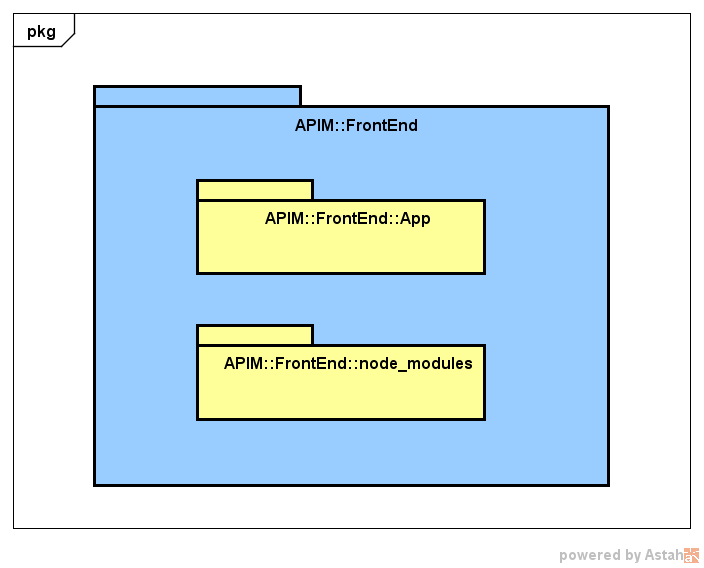
\includegraphics
	[width=0.7\linewidth]
	{images/APIM/FrontEnd/FrontEnd.png}
	\caption{APIM::FrontEnd}
\end{figure}

\begin{itemize}
	\item \textbf{Descrizione:} package contenente le componenti del lato front-end dell'applicazione web;
	\item \textbf{Packages contenuti:}
	\begin{itemize}
		\item App;
		\item node\_modules.
	\end{itemize}
\end{itemize}

\subsection{APIM::FrontEnd::App}

\subsubsection{Informazioni generali}

\begin{figure}[H]
	\centering
	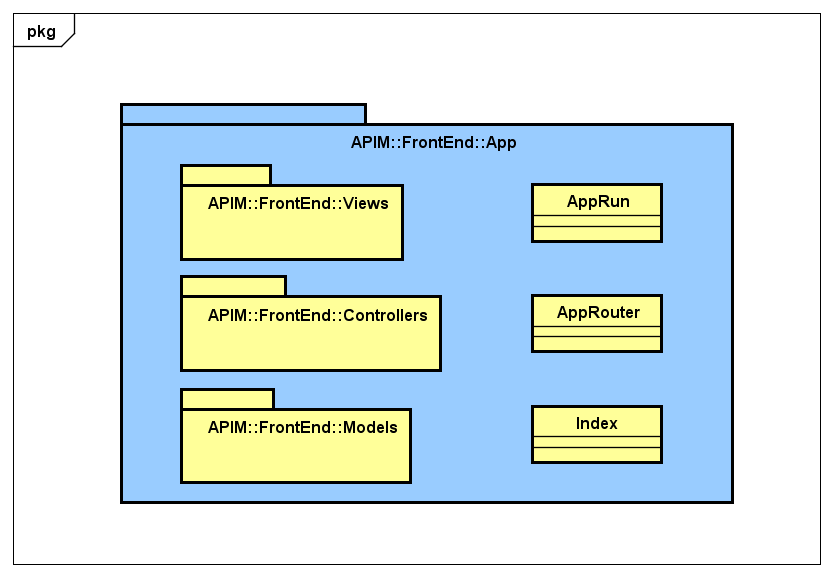
\includegraphics
	[width=0.7\linewidth]
	{images/APIM/FrontEnd/App.png}
	\caption{APIM::FrontEnd::App}
\end{figure}

\begin{itemize}
	\item \textbf{Descrizione:} Il package App contiene tutto il necessario al funzionamento del front-end dell'applicazione web API Market;
	\item \textbf{Packages contenuti:}
	\begin{itemize}
		\item Views;
		\item Models;
		\item Controllers.
	\end{itemize}
\end{itemize}

\subsubsection{Classi}

\paragraph{APIM::FrontEnd::App::AppRouter}

\begin{figure}[H]
	\centering
	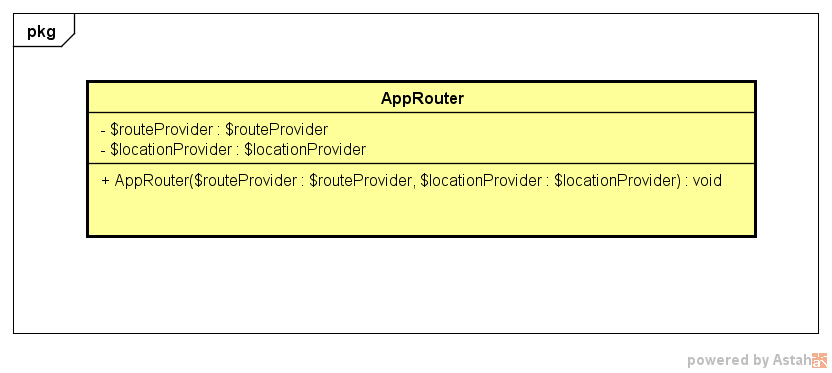
\includegraphics
	[width=0.7\linewidth]
	{images/APIM/FrontEnd/AppRouter.png}
	\caption{APIM::FrontEnd::App::AppRouter}
\end{figure}

\begin{itemize}
	\item \textbf{Descrizione:} La classe AppRouter gestisce le routes dell'applicazione, collegando le views con i rispettivi controllers attraverso i servizi di \$routeProvider e \$locationProvider;
	\item \textbf{Attributi:}
		\begin{itemize}
			\item \textbf{\$routeProvider:} \$routeProvider\\
			Campo dati con il riferimento al servizio di AngularJS dedicato al routing;
			\item \textbf{\$locationProvider:} \$locationProvider\\
			Campo dati con il riferimento al servizio di AngularJS dedicato al pathing;
		\end{itemize}
	\item \textbf{Metodi:}
		\begin{itemize}
			\item \textbf{AppRouter(\$routeProvider: \$routeProvider, \$locationProvider:
\$locationProvider):}
			Metodo per la gestione di routing e pathing dell'applicazione.
		\end{itemize}
\end{itemize}

\paragraph{APIM::FrontEnd::App::AppRun}

\begin{figure}[H]
	\centering
	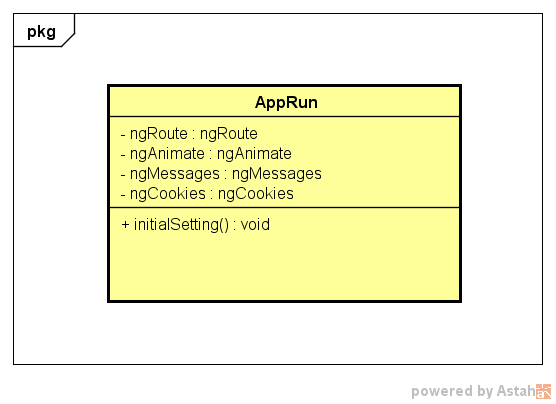
\includegraphics
	[width=0.7\linewidth]
	{images/APIM/FrontEnd/AppRun.png}
	\caption{APIM::FrontEnd::App::AppRun}
\end{figure}

\begin{itemize}
	\item \textbf{Descrizione:} La classe AppRun verifica la corretta autenticazione dell'utente e che le sue autorizzazioni gli consentano di visitare la pagina richiesta;
	\item \textbf{Attributi:}
		\begin{itemize}
			\item \textbf{ngRoute}: ngRoute\\
			Campo dati con il riferimento al modulo ngRoute di AngularJS;
			\item \textbf{ngAnimate}: ngAnimate\\
			Campo dati con il riferimento al modulo ngAnimate di AngularJS;
			\item \textbf{ngMessages}: ngMessages\\
			Campo dati con il riferimento al modulo ngMessages di AngularJS;
			\item \textbf{ngCookies}: ngCookies\\
			Campo dati con il riferimento al modulo ngCookies di AngularJS.
		\end{itemize}
	\item \textbf{Metodi:}
		\begin{itemize}
			\item \textbf{initialSetting(): void}
			Metodo per l'inizializzazione dei campi dati ai valori di default.
		\end{itemize}
	\item \textbf{Relazioni con altre classi:}
	\begin{itemize}
		\item Utilizza il modulo ngRoute per effettuare il routing dell'applicazione;
		\item Utilizza il modulo ngAnimate per impiegare transizioni ed animazioni nell'applicazione;
		\item Utilizza il modulo ngMessages per mostrare messaggi d'aiuto durante le procedure e form dell'applicazione;
		\item Utilizza il modulo ngCookies per effettuare il salvataggio dei cookies dell'applicazione.
	\end{itemize}
\end{itemize}

\paragraph{APIM::FrontEnd::App::Index}

\begin{figure}[H]
	\centering
	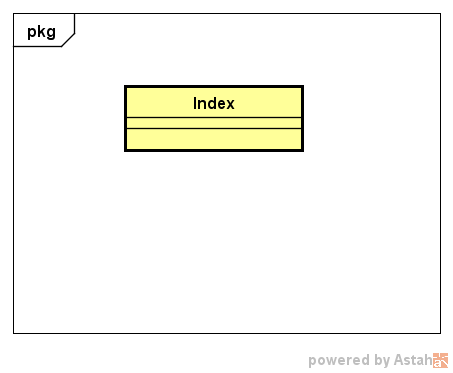
\includegraphics
	[width=0.7\linewidth]
	{images/APIM/FrontEnd/Index.png}
	\caption{APIM::FrontEnd::App::Index}
\end{figure}

\begin{itemize}
	\item \textbf{Descrizione:} La classe Index contiene la view principale dell'applicazione, dove l'utente visualizza dinamicamente le pagine che vuole visitare.
	\item \textbf{Relazioni con altre classi:}
	\begin{itemize}
		\item Interagisce con il package Views, necessario alla corretta visualizzazione delle pagine.
	\end{itemize}
\end{itemize}

% Fine App

\subsection{APIM::FrontEnd::App::Views}

\subsubsection{Informazioni generali}

\begin{figure}[H]
	\centering
	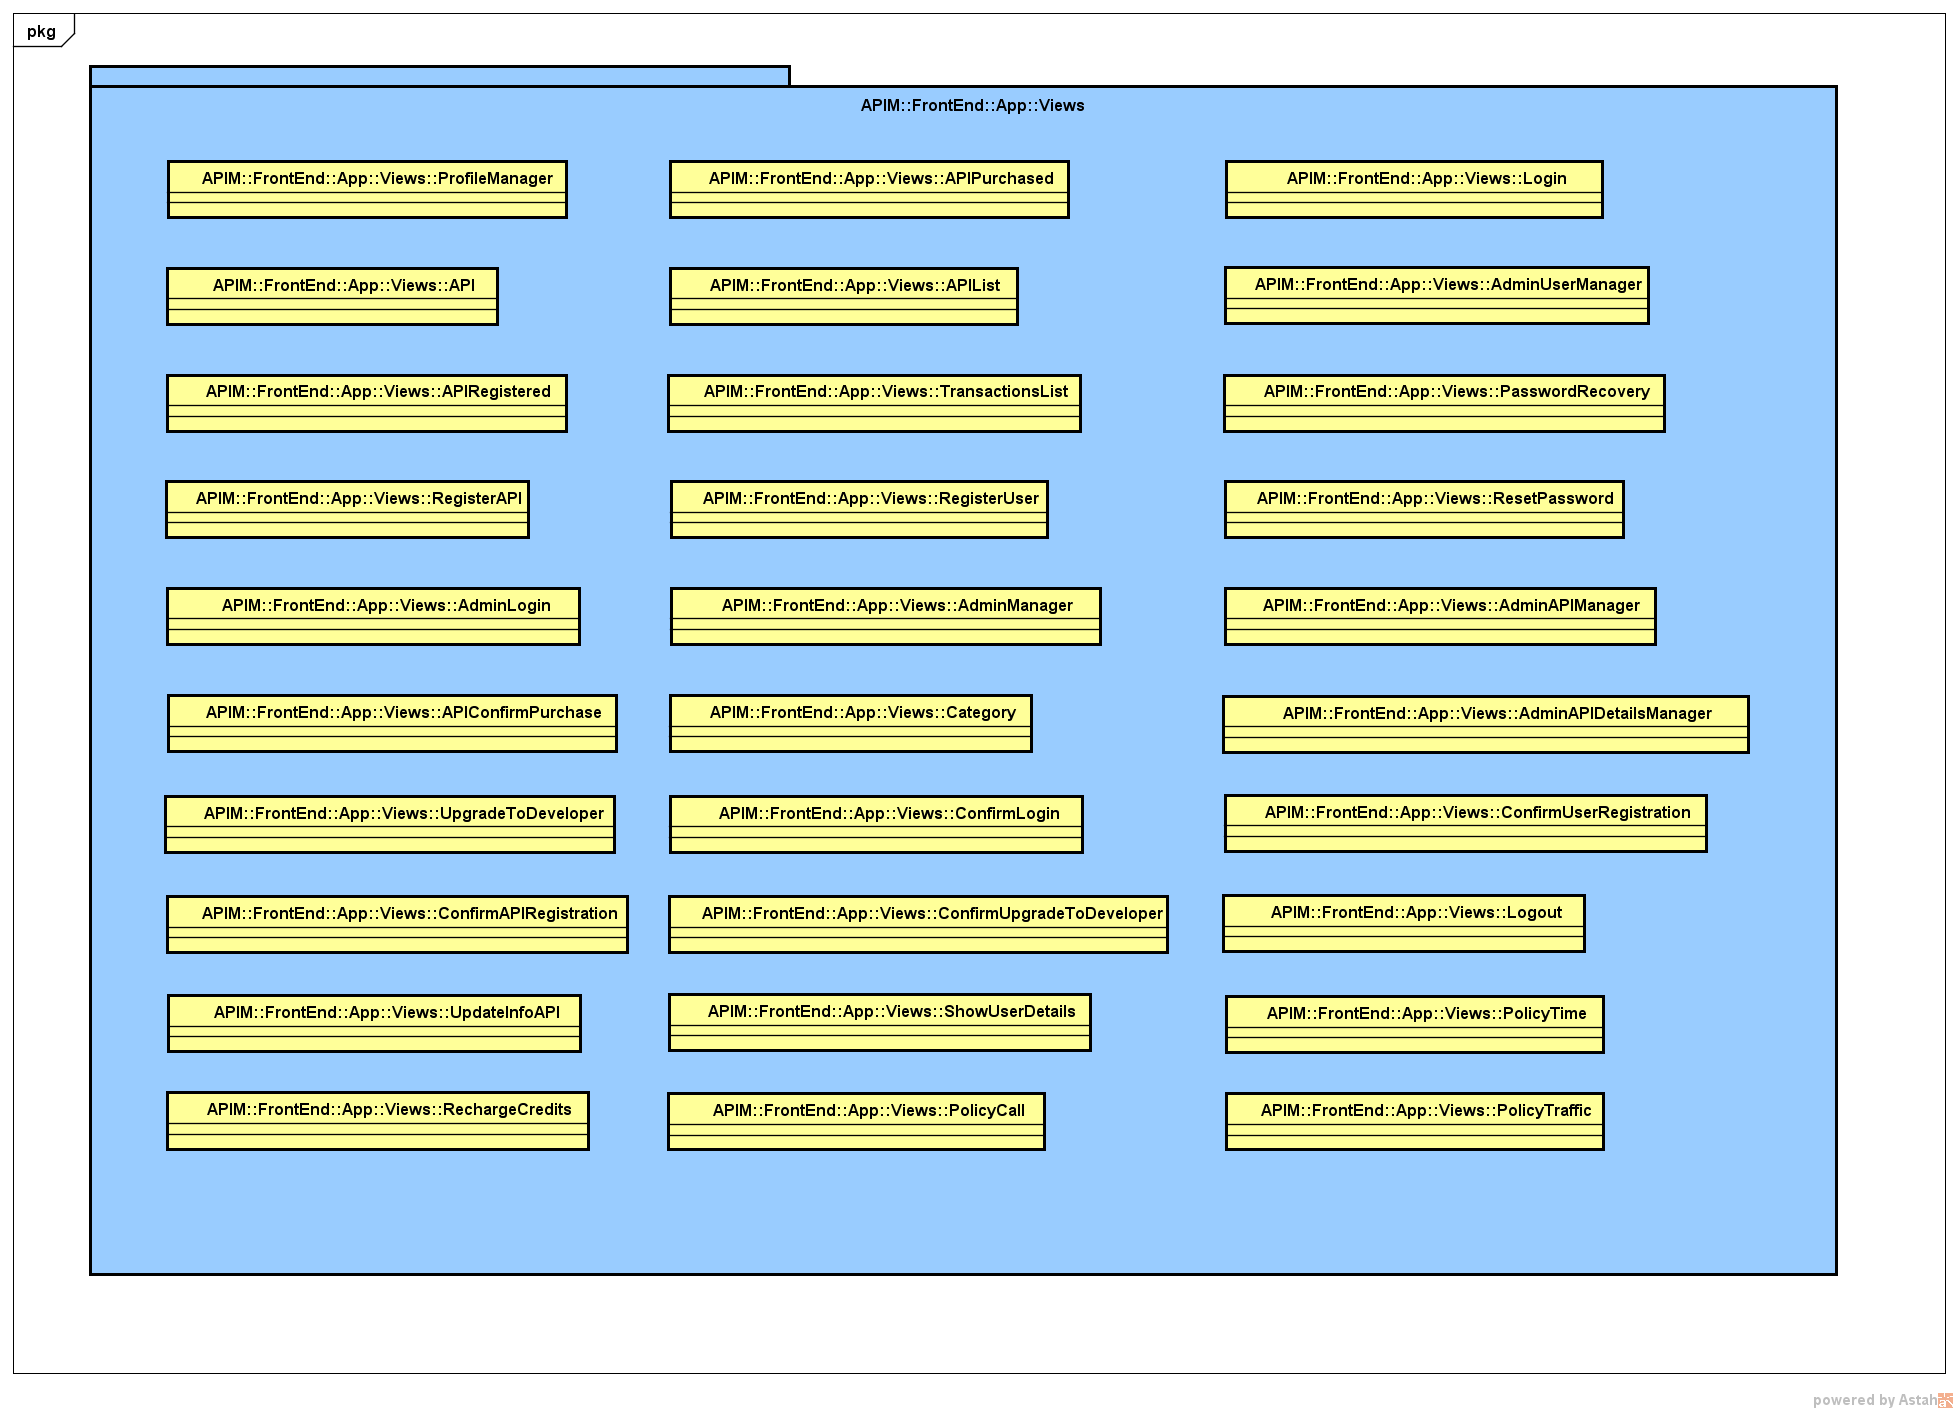
\includegraphics
	[width=0.7\linewidth]
	{images/APIM/FrontEnd/Views/views.png}
	\caption{APIM::FrontEnd::App::Views}
\end{figure}

\begin{itemize}
	\item \textbf{Descrizione:} Il package Views contiene tutte le view dell'applicazione.
	\item \textbf{Relazioni con altre classi:}
	\begin{itemize}
		\item Il package \textbf{Controllers} collega le views ad un controller per gestirne la visualizzazione da parte dell'utente; 
		\item Il package \textbf{Models} definisce le strutture dati utilizzate da views e controllers.
	\end{itemize}
\end{itemize}

\subsubsection{Classi}

\paragraph{APIM::FrontEnd::App::Views::ProfileManager}

\begin{figure}[H]
	\centering
	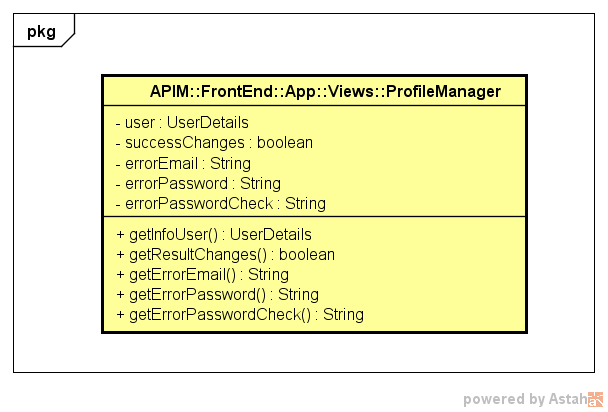
\includegraphics
	[width=0.7\linewidth]
	{images/APIM/FrontEnd/Views/ProfileManager.png}
	\caption{APIM::FrontEnd::App::Views::ProfileManager}
\end{figure}

\begin{itemize}
	\item \textbf{Descrizione:} View contenente il form dedicato alla registrazione di un utente,
il quale può inserire i campi necessari e registrarsi così alla piattaforma. Contiene,
inoltre, un link alla pagina di login;
	\item \textbf{Attributi:}
		\begin{itemize}
			\item \textbf{user : Object}\\
			Campo dati contenente le informazioni di un utente;
			\item \textbf{imageObject : Object}\\
			Campo dati contenente le informazioni dell'avatar dell'utente;
			\item \textbf{successChanges : string}\\
			Campo dati contenente la conferma delle modifiche;
			\item \textbf{errorEmail : string}\\
			Campo dati contenente l'eventuale errore di inserimento dell'email;
			\item \textbf{errorPassword : string}\\
			Campo dati contenente l'eventuale errore di inserimento della password;
			\item \textbf{errorPasswordCheck : string}\\
			Campo dati contenente l'eventuale errore della conferma della password.
		\end{itemize}
	\item \textbf{Relazioni con altre classi:}
	\begin{itemize}
		\item Interagisce con il controller \textbf{ProfileManagerController};
		\item Il model \textbf{UsersDetailModel} contiene le informazioni per rappresentare un utente.
	\end{itemize}
\end{itemize}

\paragraph{APIM::FrontEnd::App::Views::API}

\begin{figure}[H]
	\centering
	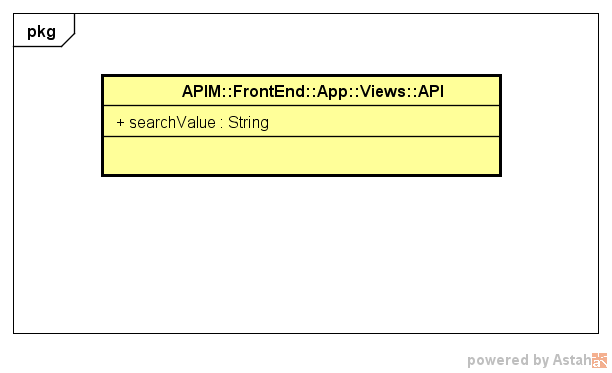
\includegraphics
	[width=0.7\linewidth]
	{images/APIM/FrontEnd/Views/API.png}
	\caption{APIM::FrontEnd::App::Views::API}
\end{figure}

\begin{itemize}
	\item \textbf{Descrizione:} View contenente i risultati della ricerca effettuata, che permette di selezionare un risultato presente al suo interno.
	\item \textbf{Attributi:}
		\begin{itemize}
			\item \textbf{searchValue : string}
			Campo dati contenente le keywords di ricerca dell'API.
		\end{itemize}
	\item \textbf{Relazioni con altre classi:}
	\begin{itemize}
		\item Interagisce con il controller \textbf{SearchController};
		\item Il model \textbf{MicroserviceModel} contiene le informazioni per rappresentare una API.
	\end{itemize}
\end{itemize}

\paragraph{APIM::FrontEnd::App::Views::APIRegistered}

\begin{figure}[H]
	\centering
	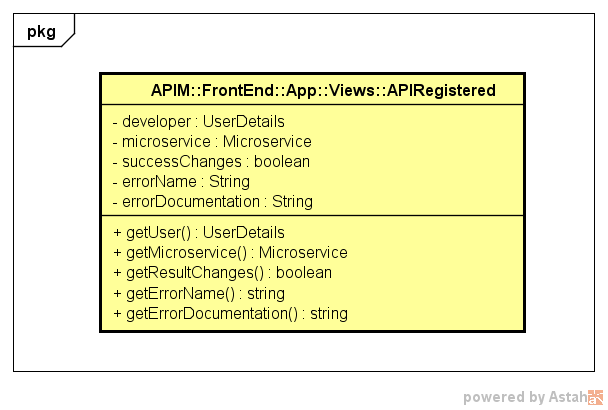
\includegraphics
	[width=0.7\linewidth]
	{images/APIM/FrontEnd/Views/APIRegistered.png}
	\caption{APIM::FrontEnd::App::Views::APIRegistered}
\end{figure}

\begin{itemize}
	\item \textbf{Descrizione:} View contenente la lista delle API registrate dall'utente sulla piattaforma.
	\item \textbf{Attributi:}
		\begin{itemize}
			\item \textbf{user : Object}\\
			Campo dati contenente le informazioni di un utente;
			\item \textbf{microservice : Object}\\
			Campo dati contenente le informazioni di un microservizio;
			\item \textbf{successChanges : string}\\
			Campo dati contenente la conferma delle modifiche;
			\item \textbf{errorName : string}\\
			Campo dati contenente l'eventuale errore di inserimento del nome;
			\item \textbf{errorDocumentation: string}\\
			Campo dati contenente l'eventuale errore di inserimento della documentazione.
		\end{itemize}
	\item \textbf{Relazioni con altre classi:}
	\begin{itemize}
		\item Interagisce con il controller \textbf{APIRegisteredController};
		\item Il model \textbf{UsersDetailModel} contiene le informazioni per rappresentare un utente;
		\item Il model \textbf{MicroserviceModel} contiene le informazioni per rappresentare una API.
	\end{itemize}
\end{itemize}

\paragraph{APIM::FrontEnd::App::Views::RegisterAPI}

\begin{figure}[H]
	\centering
	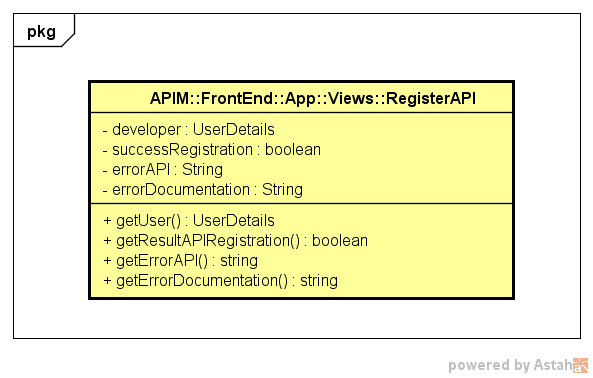
\includegraphics
	[width=0.7\linewidth]
	{images/APIM/FrontEnd/Views/RegisterAPI.png}
	\caption{APIM::FrontEnd::App::Views::RegisterAPI}
\end{figure}

\begin{itemize}
	\item \textbf{Descrizione:} View contenente il form per l'inserimento di una API da parte di un
utente sviluppatore. Lo sviluppatore può inserire tutti i dati relativi al microservizio
che intende esporre su API Market.
	\item \textbf{Attributi:}
		\begin{itemize}
			\item \textbf{user : Object}\\
			Campo dati contenente le informazioni di un utente;
			\item \textbf{microservice : Object}\\
			Campo dati contenente le informazioni di una API;
			\item \textbf{successRegistration : string}\\
			Campo dati contenente la conferma della registrazione;
			\item \textbf{errorAPI : string}\\
			Campo dati contenente l'eventuale errore di inserimento dell'API;
			\item \textbf{errorDocumentation: string}\\
			Campo dati contenente l'eventuale errore di inserimento della documentazione.
		\end{itemize}
	\item \textbf{Relazioni con altre classi:}
	\begin{itemize}
		\item Interagisce con il controller \textbf{APIRegistrationController};
		\item Il model \textbf{UsersDetailModel} contiene le informazioni per rappresentare un utente;
		\item Il model \textbf{MicroserviceModel} contiene le informazioni per rappresentare una API.
	\end{itemize}
\end{itemize}

\paragraph{APIM::FrontEnd::App::Views::SellingPolicy}

\begin{figure}[H]
	\centering
	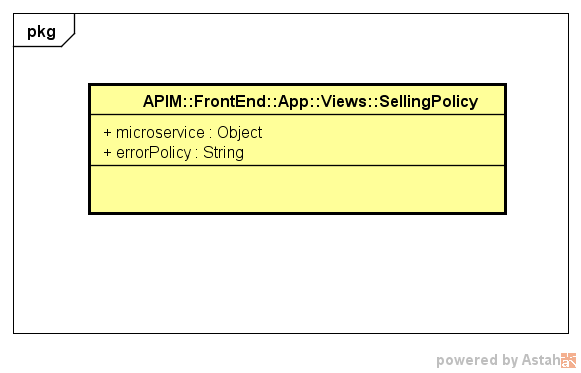
\includegraphics
	[width=0.7\linewidth]
	{images/APIM/FrontEnd/Views/SellingPolicy.png}
	\caption{APIM::FrontEnd::App::Views::SellingPolicy}
\end{figure}

\begin{itemize}
	\item \textbf{Descrizione:} View contenente il form per la gestione delle differenti policy di vendita
per un singolo microservizio.
	\item \textbf{Attributi:}
		\begin{itemize}
			\item \textbf{microservice : Object}\\
			Campo dati contenente le informazioni di una API;
			\item \textbf{errorPolicy : string}\\
			Campo dati contenente l'eventuale errore di inserimento della policy di vendita.
		\end{itemize}
	\item \textbf{Relazioni con altre classi:}
	\begin{itemize}
		\item Interagisce con il controller \textbf{SellingPolicyController};
		\item Il model \textbf{MicroserviceModel} contiene le informazioni per rappresentare una API.
	\end{itemize}
\end{itemize}

\paragraph{APIM::FrontEnd::App::Views::APIPurchased}

\begin{figure}[H]
	\centering
	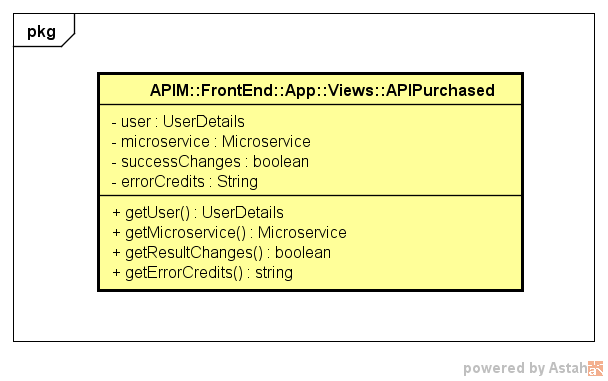
\includegraphics
	[width=0.7\linewidth]
	{images/APIM/FrontEnd/Views/APIPurchased.png}
	\caption{APIM::FrontEnd::App::Views::APIPurchased}
\end{figure}

\begin{itemize}
	\item \textbf{Descrizione:} View contenente la lista delle API acquistate da un utente della piattaforma API Market.
	\item \textbf{Attributi:}
		\begin{itemize}
			\item \textbf{user : Object}\\
			Campo dati contenente le informazioni di un utente;
			\item \textbf{microservice : Object}\\
			Campo dati contenente le informazioni di una API;
			\item \textbf{successChanges : string}\\
			Campo dati contenente la conferma del rinnovo dell'API;
			\item \textbf{errorCredits : string}\\
			Campo dati contenente l'eventuale errore di rinnovo dell'API.
		\end{itemize}
	\item \textbf{Relazioni con altre classi:}
	\begin{itemize}
		\item Interagisce con il controller \textbf{APIPurchasedController};
		\item Il model \textbf{UserDetailsModel} contiene le informazioni per rappresentare un utente;
		\item Il model \textbf{TransactionModel} contiene le informazioni per rappresentare una transazione;
		\item Il model \textbf{MicroserviceModel} contiene le informazioni per rappresentare una API.
	\end{itemize}
\end{itemize}

\paragraph{APIM::FrontEnd::App::Views::APIList}

\begin{figure}[H]
	\centering
	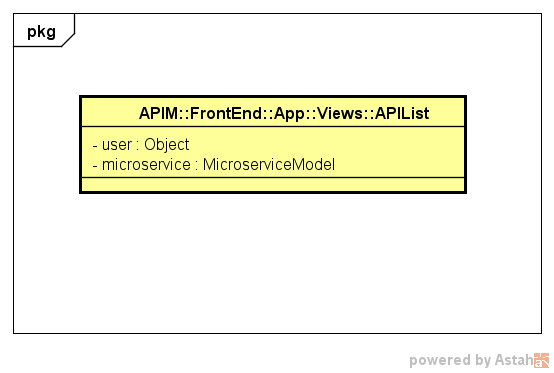
\includegraphics
	[width=0.7\linewidth]
	{images/APIM/FrontEnd/Views/APIList.png}
	\caption{APIM::FrontEnd::App::Views::APIList}
\end{figure}

\begin{itemize}
	\item \textbf{Descrizione:} View contenente la lista delle API in seguito ad una ricerca.
	\item \textbf{Attributi:}
	\begin{itemize}
		\item \textbf{user : Object}\\
		Campo dati contenente le informazioni di un utente;
		\item \textbf{microservice : Object}\\
		Campo dati contenente le informazioni di una API.
	\end{itemize}
	\item \textbf{Relazioni con altre classi:}
	\begin{itemize}
		\item Interagisce con il controller \textbf{APIListController};
		\item Il model \textbf{UserDetailsModel} contiene le informazioni per rappresentare un utente;
		\item Il model \textbf{MicroserviceModel} contiene le informazioni per rappresentare una API.
	\end{itemize}
\end{itemize}

\paragraph{APIM::FrontEnd::App::Views::TransactionsList}

\begin{figure}[H]
	\centering
	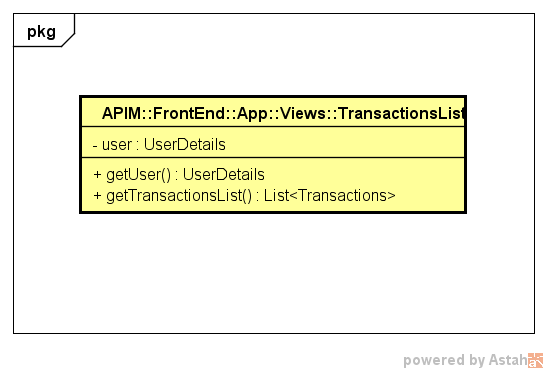
\includegraphics
	[width=0.7\linewidth]
	{images/APIM/FrontEnd/Views/TransactionsList.png}
	\caption{APIM::FrontEnd::App::Views::TransactionsList}
\end{figure}

\begin{itemize}
	\item \textbf{Descrizione:} View contenente l'elenco delle transazioni effettuate da un utente
su API Market.
	\item \textbf{Attributi:}
	\begin{itemize}
		\item \textbf{user : Object}\\
		Campo dati contenente le informazioni di un utente.
	\end{itemize}
	\item \textbf{Relazioni con altre classi:}
	\begin{itemize}
		\item Interagisce con il controller \textbf{TransactionsListController};
		\item Il model \textbf{TransactionModel} contiene le informazioni per rappresentare una API.
	\end{itemize}
\end{itemize}

\paragraph{APIM::FrontEnd::App::Views::RegisterUser}

\begin{figure}[H]
	\centering
	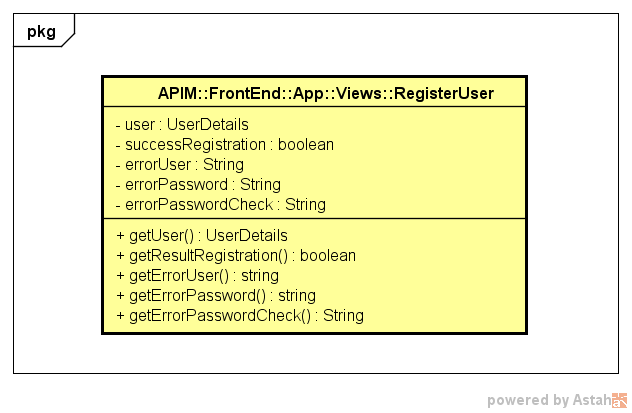
\includegraphics
	[width=0.7\linewidth]
	{images/APIM/FrontEnd/Views/RegisterUser.png}
	\caption{APIM::FrontEnd::App::Views::RegisterUser}
\end{figure}

\begin{itemize}
	\item \textbf{Descrizione:} View contenente il form dedicato alla registrazione di un utente, il
quale può inserire i campi necessari e registrarsi così alla piattaforma. Contiene,
inoltre, un link alla pagina di login;
	\item \textbf{Attributi:}
	\begin{itemize}
		\item \textbf{user : Object}\\
		Campo dati contenente le informazioni di un utente;
		\item \textbf{successRegistration : string}\\
		Campo dati contenente il messaggio di successo della registrazione;
		\item \textbf{errorUser : string}\\
		Campo dati contenente l'eventuale errore di inserimento delle informazioni dell'utente;
		\item \textbf{errorPassword : string}\\
		Campo dati contenente l'eventuale errore di inserimento della password;
		\item \textbf{errorPasswordCheck : string}\\
		Campo dati contenente l'eventuale errore di reinserimento della password.
	\end{itemize}
	\item \textbf{Relazioni con altre classi:}
	\begin{itemize}
		\item Interagisce con il controller \textbf{RegisterUserController};
		\item Il model \textbf{UserDetailsModel} contiene le informazioni per rappresentare un utente.
	\end{itemize}
\end{itemize}

\paragraph{APIM::FrontEnd::App::Views::AdminManager}

\begin{figure}[H]
	\centering
	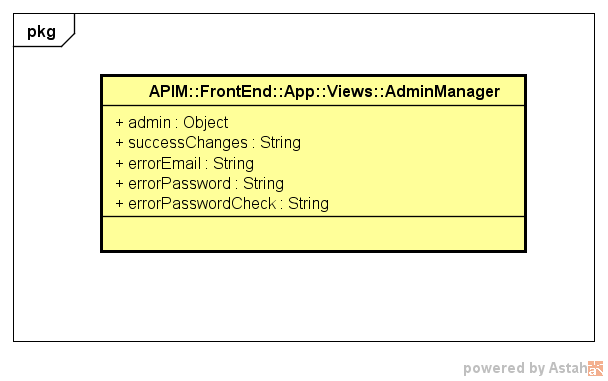
\includegraphics
	[width=0.7\linewidth]
	{images/APIM/FrontEnd/Views/AdminManager.png}
	\caption{APIM::FrontEnd::App::Views::AdminManager}
\end{figure}

\begin{itemize}
	\item \textbf{Descrizione:} View contenente le operazioni per la gestione del profilo amministratore
API Market.
	\item \textbf{Attributi:}
	\begin{itemize}
		\item \textbf{user : Object}\\
		Campo dati contenente le informazioni di un utente;
		\item \textbf{successChanges : string}\\
		Campo dati contenente il messaggio di successo delle modifiche;
		\item \textbf{errorUser : string}\\
		Campo dati contenente l'eventuale errore di inserimento delle informazioni dell'utente;
		\item \textbf{errorPassword : string}\\
		Campo dati contenente l'eventuale errore di inserimento della password;
		\item \textbf{errorPasswordCheck : string}\\
		Campo dati contenente l'eventuale errore di reinserimento della password.
	\end{itemize}
	\item \textbf{Relazioni con altre classi:}
	\begin{itemize}
		\item Interagisce con il controller \textbf{AdminManagerController};
		\item Il model \textbf{UserDetailsModel} contiene le informazioni per rappresentare un utente.
	\end{itemize}
\end{itemize}

\paragraph{APIM::FrontEnd::App::Views::Login}

\begin{figure}[H]
	\centering
	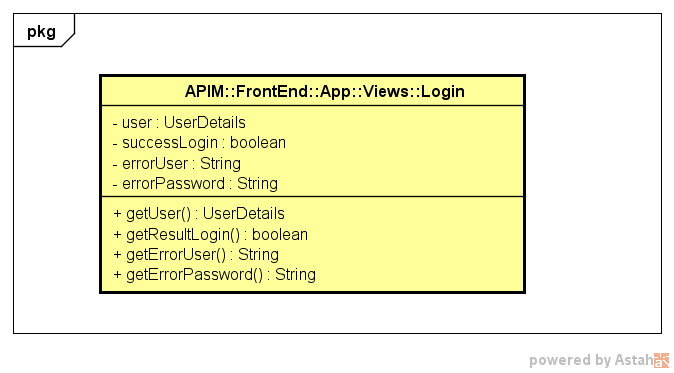
\includegraphics
	[width=0.7\linewidth]
	{images/APIM/FrontEnd/Views/Login.png}
	\caption{APIM::FrontEnd::App::Views::Login}
\end{figure}

\begin{itemize}
	\item \textbf{Descrizione:} View contenente il form necessario affinchè l'utente possa effettuare il login ed autenticarsi al sistema. Contiene, inoltre, un link alla pagina di registrazione e uno alla pagina per il recupero della password
	\item \textbf{Attributi:}
	\begin{itemize}
		\item \textbf{user : Object}\\
		Campo dati contenente le informazioni di un utente;
		\item \textbf{successLogin : string}\\
		Campo dati contenente il messaggio di successo del login;
		\item \textbf{errorUser : string}\\
		Campo dati contenente l'eventuale errore di inserimento delle informazioni dell'utente;
		\item \textbf{errorPassword : string}\\
		Campo dati contenente l'eventuale errore di inserimento della password.
	\end{itemize}
	\item \textbf{Relazioni con altre classi:}
	\begin{itemize}
		\item Interagisce con il controller \textbf{LoginController};
		\item Il model \textbf{UserDetailsModel} contiene le informazioni per rappresentare un utente.
	\end{itemize}
\end{itemize}

\paragraph{APIM::FrontEnd::App::Views::VirtualAccount}

\begin{figure}[H]
	\centering
	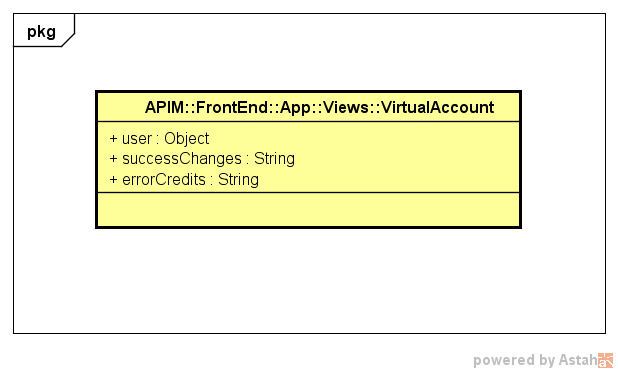
\includegraphics
	[width=0.7\linewidth]
	{images/APIM/FrontEnd/Views/VirtualAccount.png}
	\caption{APIM::FrontEnd::App::Views::VirtualAccount}
\end{figure}

\begin{itemize}
	\item \textbf{Descrizione:} View contenente le informazioni relative al conto virtuale personale
associato al profilo utente.
	\item \textbf{Attributi:}
	\begin{itemize}
		\item \textbf{user : Object}\\
		Campo dati contenente le informazioni di un utente;
		\item \textbf{successChanges : string}\\
		Campo dati contenente il messaggio di successo della ricarica crediti;
		\item \textbf{errorCredits : string}\\
		Campo dati contenente l'eventuale errore di acquisto crediti.
	\end{itemize}
	\item \textbf{Relazioni con altre classi:}
	\begin{itemize}
		\item Interagisce con il controller \textbf{VirtualAccountController};
		\item Il model \textbf{UserDetailsModel} contiene le informazioni per rappresentare un utente;
		\item Il model \textbf{TransactionModel} contiene le informazioni per rappresentare una transazione.
	\end{itemize}
\end{itemize}

\paragraph{APIM::FrontEnd::App::Views::PasswordRecovery}

\begin{figure}[H]
	\centering
	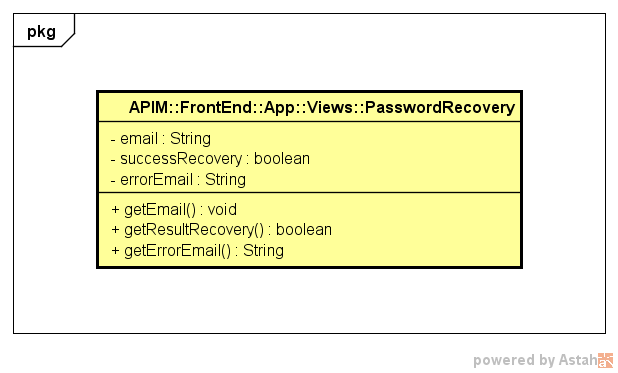
\includegraphics
	[width=0.7\linewidth]
	{images/APIM/FrontEnd/Views/PasswordRecovery.png}
	\caption{APIM::FrontEnd::App::Views::PasswordRecovery}
\end{figure}

\begin{itemize}
	\item \textbf{Descrizione:} View contenente il form dedicato al recupero della password di un utente, il quale può inserire l'indirizzo email e ricevere una nuova password con la quale autenticarsi al sistema. Contiene, inoltre, un link alla pagina di login;
	\item \textbf{Attributi:}
	\begin{itemize}
		\item \textbf{email : string}\\
		Campo dati contenente un indirizzo email;
		\item \textbf{successRecovery : string}\\
		Campo dati contenente il messaggio di successo del recupero password;
		\item \textbf{errorEmail : string}\\
		Campo dati contenente l'eventuale errore di inserimento dell'indirizzo email.
	\end{itemize}
	\item \textbf{Relazioni con altre classi:}
	\begin{itemize}
		\item Interagisce con il controller \textbf{PasswordRecoveryController};
		\item Il model \textbf{UserDetailsModel} contiene le informazioni per rappresentare un utente.
	\end{itemize}
\end{itemize}

\paragraph{APIM::FrontEnd::App::Views::ResetPassword}

\begin{figure}[H]
	\centering
	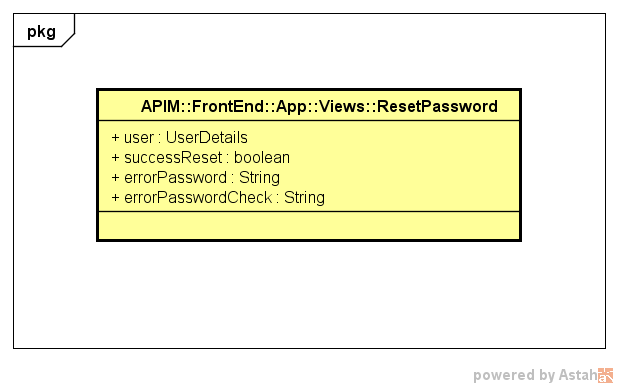
\includegraphics
	[width=0.7\linewidth]
	{images/APIM/FrontEnd/Views/ResetPassword.png}
	\caption{APIM::FrontEnd::App::Views::ResetPassword}
\end{figure}

\begin{itemize}
	\item \textbf{Descrizione:} View contenente il form dedicato al cambio di password di un utente
autenticato, il quale può inserire la nuova password che intende utilizzare per i futuri login al sistema.
	\item \textbf{Attributi:}
	\begin{itemize}
		\item \textbf{user : Object}\\
		Campo dati contenente le informazioni di un utente;
		\item \textbf{successReset : string}\\
		Campo dati contenente il messaggio di successo del reset password;
		\item \textbf{errorPassword : string}\\
		Campo dati contenente l'eventuale errore di inserimento della password.
		\item \textbf{errorPasswordCheck : string}\\
		Campo dati contenente l'eventuale errore di reinserimento della password.
	\end{itemize}
	\item \textbf{Relazioni con altre classi:}
	\begin{itemize}
		\item Interagisce con il controller \textbf{ResetPasswordController};
		\item Il model \textbf{UserDetailsModel} contiene le informazioni per rappresentare un utente.
	\end{itemize}
\end{itemize}

\paragraph{APIM::FrontEnd::App::Views::AdminModeration}

\begin{figure}[H]
	\centering
	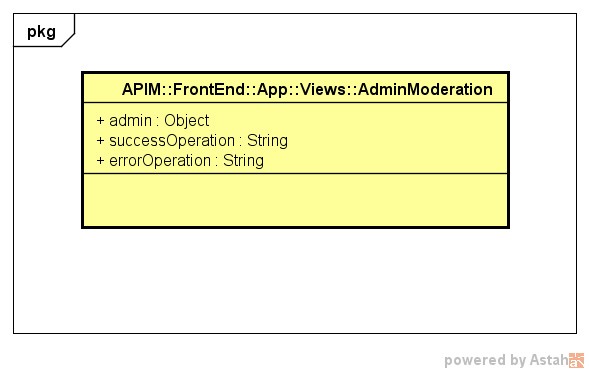
\includegraphics
	[width=0.7\linewidth]
	{images/APIM/FrontEnd/Views/AdminModeration.png}
	\caption{APIM::FrontEnd::App::Views::AdminModeration}
\end{figure}

\begin{itemize}
	\item \textbf{Descrizione:} View contenente il form dedicato alla moderazione di un utente o di una API da parte di un amministratore della piattaforma API Market.
	\item \textbf{Attributi:}
	\begin{itemize}
		\item \textbf{admin : Object}\\
		Campo dati contenente le informazioni di un utente;
		\item \textbf{successOperation : string}\\
		Campo dati contenente il messaggio di successo dell'operazione di moderazione;
		\item \textbf{errorOperation : string}\\
		Campo dati contenente l'eventuale errore dell'operazione di moderazione.
	\end{itemize}
	\item \textbf{Relazioni con altre classi:}
	\begin{itemize}
		\item Interagisce con il controller \textbf{AdminModerationController};
		\item Il model \textbf{UserDetailsModel} contiene le informazioni per rappresentare un utente.
	\end{itemize}
\end{itemize}


%Fine views

\subsection{APIM::FrontEnd::App::Models}

\subsubsection{Informazioni generali}

\begin{figure}[H]
	\centering
	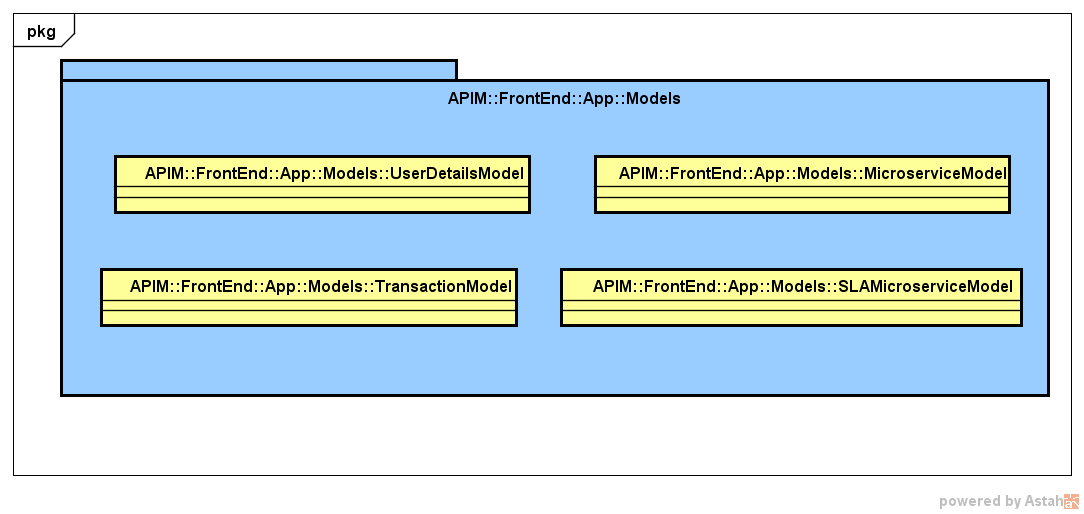
\includegraphics
	[width=0.7\linewidth]
	{images/APIM/FrontEnd/Models/Models.png}
	\caption{APIM::FrontEnd:App:Models}
\end{figure}

\begin{itemize}
	\item \textbf{Descrizione:} Il package Models contiene le classi che definiscono le strutture dei dati di utenti, microservizi, transazioni e sondaggi SLA.
	\item \textbf{Relazioni con altre classi:}
		\begin{itemize}
			\item Interagisce con i package \textbf{Controllers} e \textbf{Views} per garantire il dynamic binding di AngularJS.
		\end{itemize}
\end{itemize}

\subsubsection{Classi}

\paragraph{APIM::FrontEnd::App::Models::UserDetailsModel}

\begin{figure}[H]
	\centering
	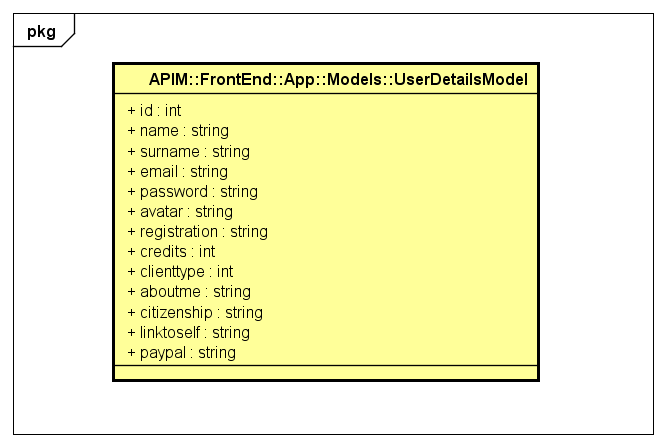
\includegraphics
	[width=0.7\linewidth]
	{images/APIM/FrontEnd/Models/UserDetailsModel.png}
	\caption{APIM::FrontEnd::App::Models:UserDetailsModel}
\end{figure}

\begin{itemize}
	\item \textbf{Descrizione:} UserDetailsModel che rappresenta un utente e che contiene tutte le informazioni
necessarie alla presentazione del contenuto di un utente, sia nella visualizzazione che nella gestione di un profilo.
	\item \textbf{Attributi:}
		\begin{itemize}
			\item \textbf{id : int}\\
			Id dell'utente;
			\item \textbf{name : string}\\
			Nome dell'utente;
			\item \textbf{surname : string}\\
			Cognome dell'utente;
			\item \textbf{email : string}\\
			Email dell'utente;
			\item \textbf{password : string}\\
			Password dell'utente;
			\item \textbf{avatar : string}\\
			Avatar dell'utente;
			\item \textbf{registration : string}\\
			Data di registrazione dell'utente;
			\item \textbf{credits : int}\\
			Crediti dell'utente;
			\item \textbf{clienttype : int}\\
			Tipo di account dell'utente;
			\item \textbf{aboutme : string}\\
			AboutMe dell'utente sviluppatore;
			\item \textbf{citizenship : string}\\
			Cittadinanza dell'utente sviluppatore;
			\item \textbf{linktoself : string}\\
			Link al sito esterno dell'utente sviluppatore;
			\item \textbf{paypal : string}\\
			Email paypal dell'utente sviluppatore.
		\end{itemize}
	\item \textbf{Relazioni con altre classi:}
		\begin{itemize}
			\item Interagisce con il controller \textbf{LoginController};
			\item Interagisce con il controller \textbf{SearchController};
			\item Interagisce con il controller \textbf{ProfileManagerController};
			\item Interagisce con il controller \textbf{ResetPasswordController};
			\item Interagisce con il controller \textbf{PasswordRecoveryController};
			\item Interagisce con il controller \textbf{Controller};
			\item Interagisce con il controller \textbf{VirtualAccountController}.
	\end{itemize}
\end{itemize}

\paragraph{APIM::FrontEnd::App::Models::TransactionModel}

\begin{figure}[H]
	\centering
	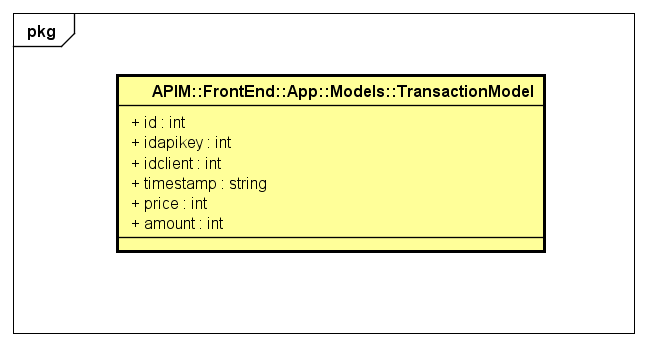
\includegraphics
	[width=0.7\linewidth]
	{images/APIM/FrontEnd/Models/TransactionModel.png}
	\caption{APIM::FrontEnd::App::Models::TransactionModel}
\end{figure}

\begin{itemize}
	\item \textbf{Descrizione:} TransactionModel rappresenta una transazione avvenuta e che contiene
tutte le informazioni necessarie alla presentazione del contenuto di una transazione,
sia nella visualizzazione che nella gestione.
	\item \textbf{Attributi:}
		\begin{itemize}
			\item \textbf{id : int}\\
			Id della transazione;
			\item \textbf{idapikey : int}\\
			Id dell'apikey;
			\item \textbf{idclient : int}\\
			Id del cliente;
			\item \textbf{timestamp : int}\\
			Data ed ora della transazione;
			\item \textbf{price : int}\\
			Prezzo della transazione;
			\item \textbf{amount : int}\\
			Ammontare quantitativo della transazione.
		\end{itemize}
	\item \textbf{Relazioni con altre classi:}
		\begin{itemize}
			\item Interagisce con il controller \textbf{TransactionsListController};
			\item Interagisce con il controller \textbf{APIPurchasedController}.
		\end{itemize}
\end{itemize}

\paragraph{APIM::FrontEnd::App::Models::MicroserviceModel}

\begin{figure}[H]
	\centering
	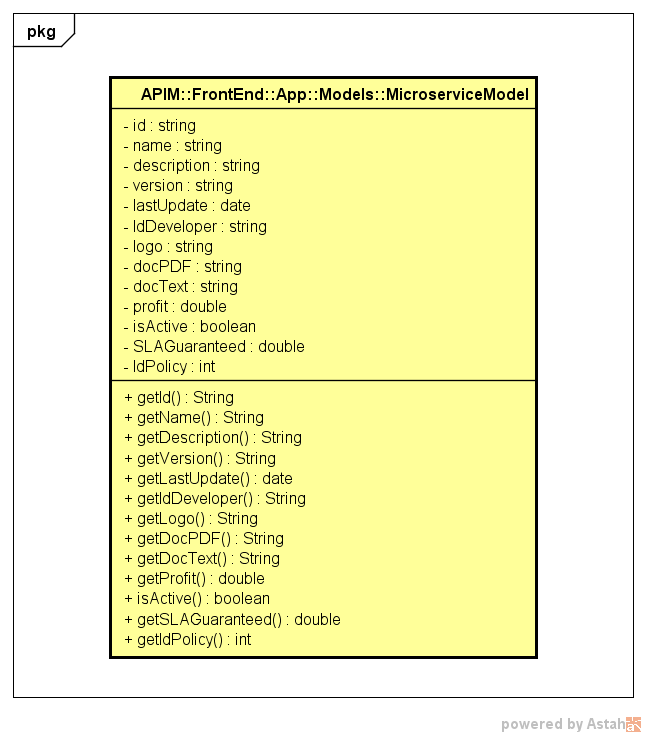
\includegraphics
	[width=0.7\linewidth]
	{images/APIM/FrontEnd/Models/MicroserviceModel.png}
	\caption{APIMarket::FrontEnd::App::Models::MicroserviceModel}
\end{figure}

\begin{itemize}
	\item \textbf{Descrizione:} MicroserviceModel rappresenta un microservizio e che contiene tutte le
informazioni necessarie alla presentazione del contenuto di un microservizio, sia nella visualizzazione che nella gestione.
	\item \textbf{Attributi:}
		\begin{itemize}
			\item \textbf{id : int}\\
			Id del microservizio;
			\item \textbf{name : string}\\
			Nome del microservizio;
			\item \textbf{description : string}\\
			Descrizione del microservizio;
			\item \textbf{version : string}\\
			Versione corrente del microservizio;
			\item \textbf{lastupdate : string}\\
			Data ultimo aggiornamento del microservizio;
			\item \textbf{iddeveloper : string}\\
			Id dello sviluppatore del microservizio;
			\item \textbf{logo : string}\\
			Link al logo del microservizio;
			\item \textbf{docpdf : string}\\
			Link al file PDF del microservizio;
			\item \textbf{docext : string}\\
			Link alla documentazione esterna del microservizio;
			\item \textbf{profit : int}\\
			Percentuale profitto dello sviluppatore del microservizio;
			\item \textbf{isactive : bool}\\
			Funzionamento attuale del microservizio;
			\item \textbf{slaguaranteed : double}\\
			SLA garantita dal microservizio;
			\item \textbf{idpolicy : int}\\
			Id della policy di vendita del microservizio.
		\end{itemize}
	\item \textbf{Relazioni con altre classi:}
		\begin{itemize}
			\item Interagisce con il controller \textbf{APIRegiteredController};
			\item Interagisce con il controller \textbf{APIRegistrationController};
			\item Interagisce con il controller \textbf{SellingPolicyController};
			\item Interagisce con il controller \textbf{APIPurchasedController};
			\item Interagisce con il controller \textbf{APIListController}.
		\end{itemize}
\end{itemize}

\paragraph{APIM::FrontEnd::App::Models::SLAMicroserviceModel}

\begin{figure}[H]
	\centering
	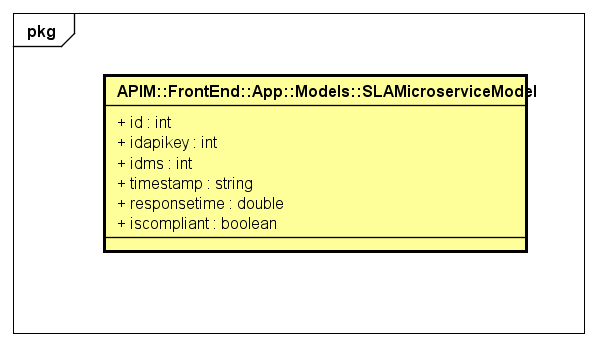
\includegraphics
	[width=0.7\linewidth]
	{images/APIM/FrontEnd/Models/SLAMicroserviceModel.png}
	\caption{APIM::FrontEnd::App::Models::SLAMicroserviceModel}
\end{figure}

\begin{itemize}
	\item \textbf{Descrizione:} SLAMicroserviceModel rappresenta la SLA di un microservizio e che
contiene tutte le informazioni necessarie alla presentazione del contenuto di SLA di un microservizio, sia nella visualizzazione che nella gestione.
	\item \textbf{Attributi:}
		\begin{itemize}
			\item \textbf{id : int}\\
			Id del sondaggio SLA;
			\item \textbf{idapikey : int}\\
			Id dell'apike attribuita al sondaggio SLA;
			\item \textbf{idms : int}\\
			Id del microservizio attribuito al sondaggio SLA;
			\item \textbf{timestamp : string}\\
			Data ed ora del sondaggio SLA;
			\item \textbf{responsetime : int}\\
			Tempo di risposta del sondaggio SLA;
			\item \textbf{iscompliant : boolean}\\
			Indicatore del rispetto del sondaggio SLA.
		\end{itemize}
	\item \textbf{Relazioni con altre classi:}
		\begin{itemize}
			\item Interagisce con il controller \textbf{SellingPolicyController};
			\item Interagisce con il controller \textbf{APIRegistrationController}.		
		\end{itemize}
\end{itemize}

%Fine models

\subsection{APIM::FrontEnd::App::Controllers}

\subsubsection{Informazioni generali}

\begin{figure}[H]
	\centering
	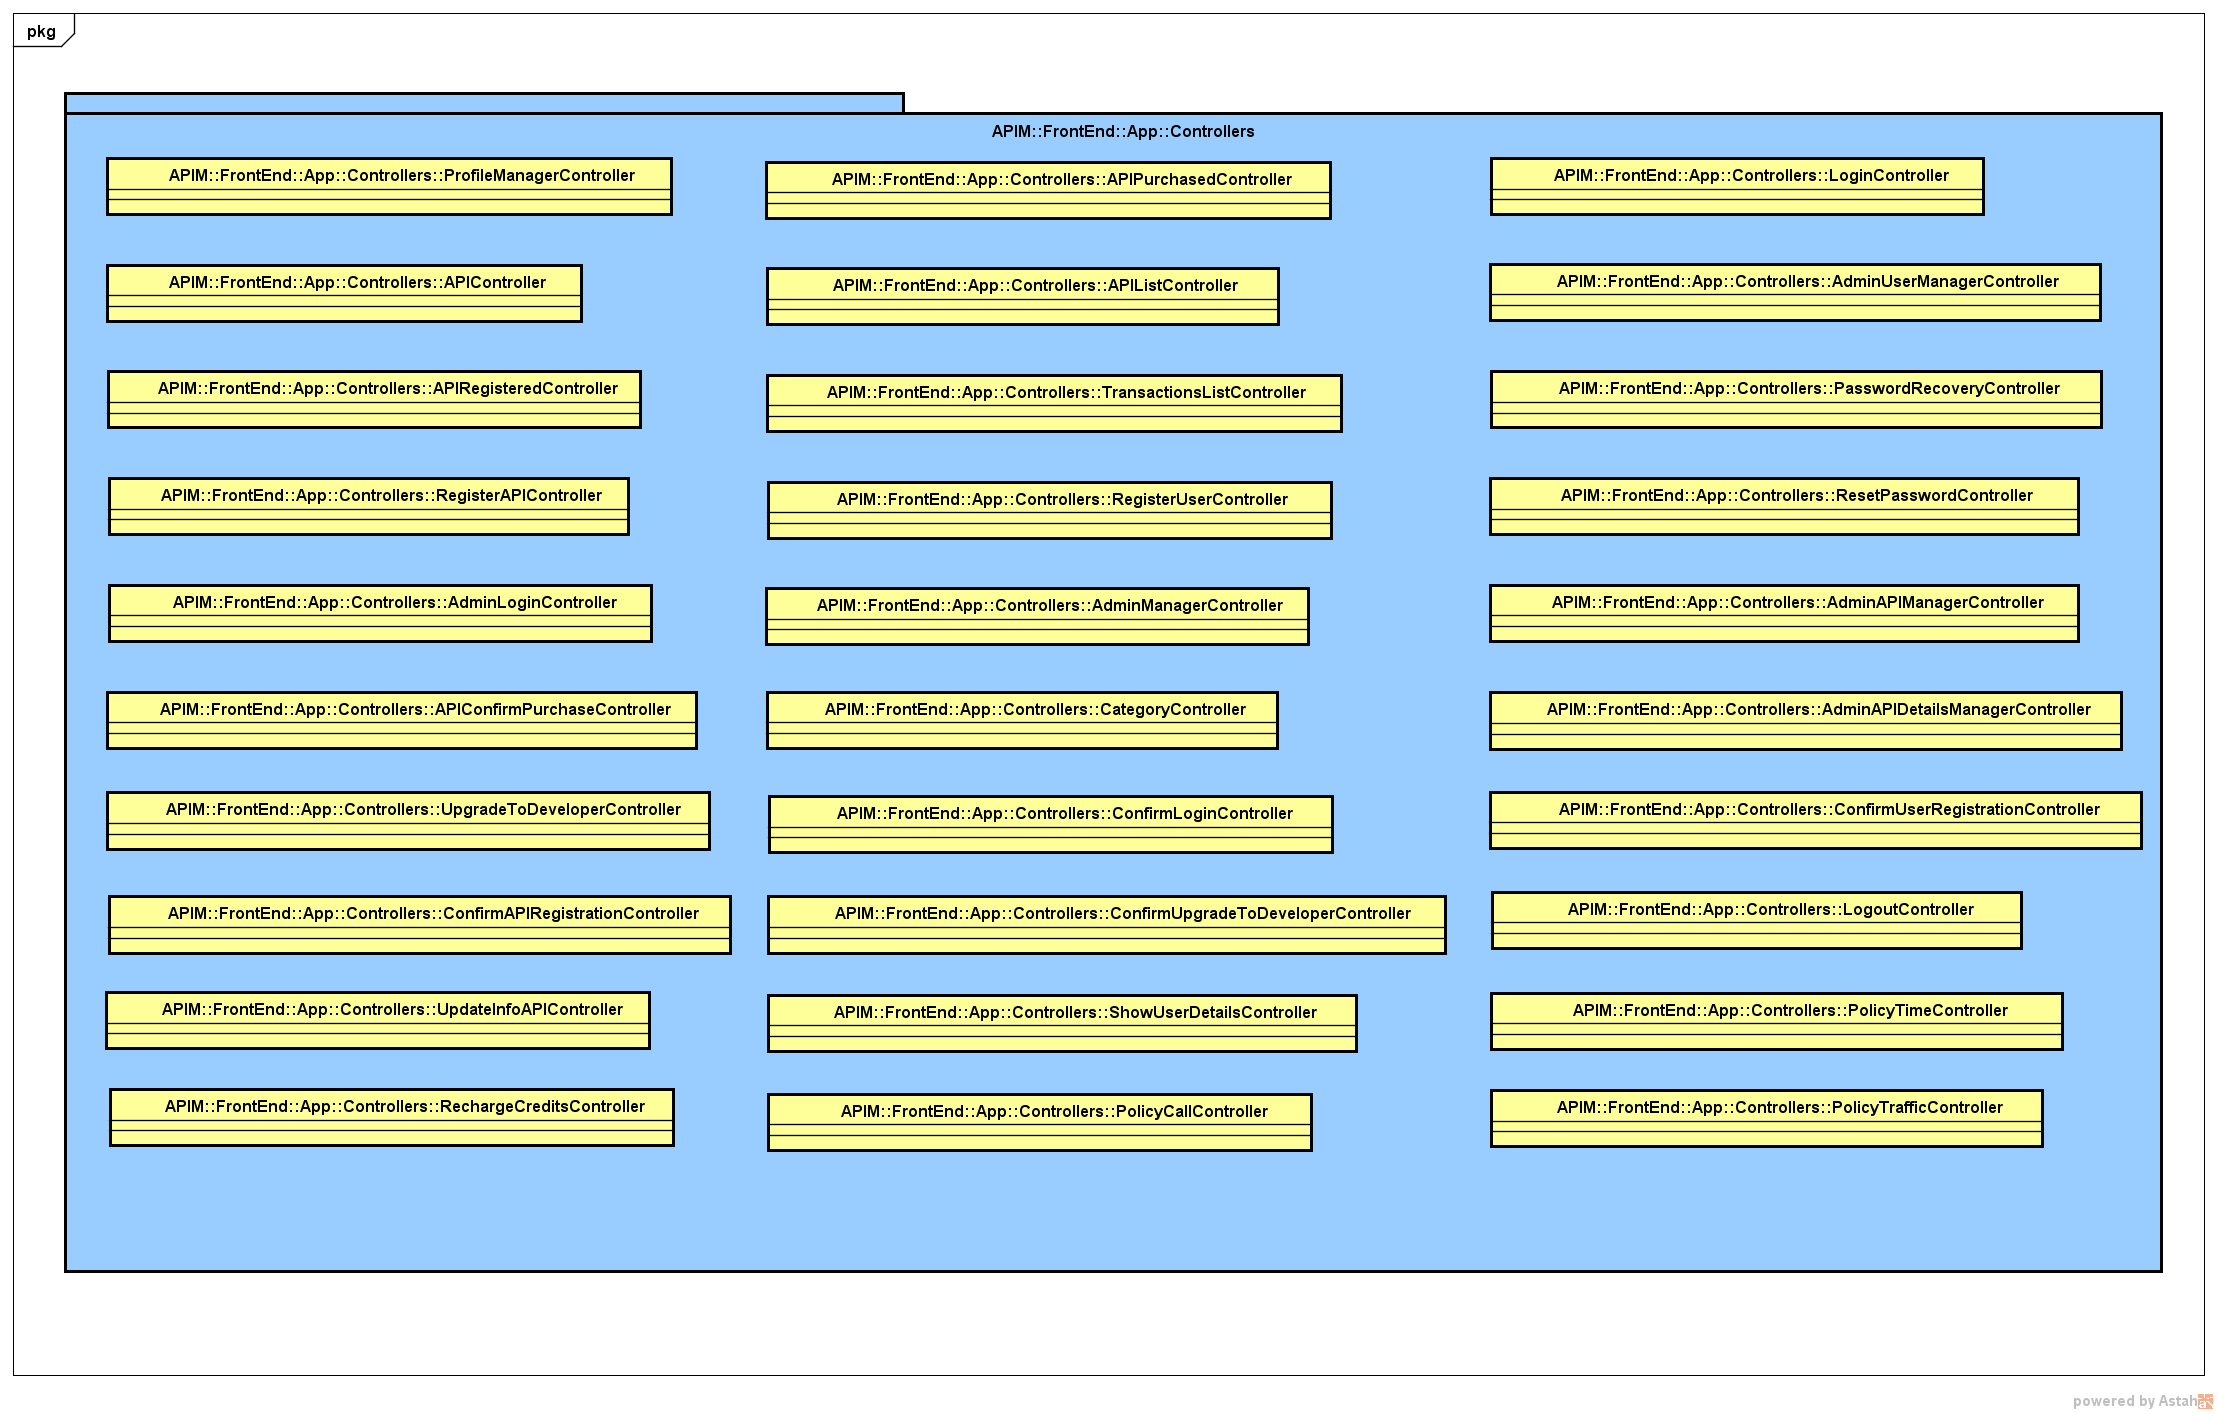
\includegraphics
	[width=0.7\linewidth]
	{images/APIM/FrontEnd/Controllers/Controllers.png}
	\caption{APIM::FrontEnd::App::Controllers}
\end{figure}

\begin{itemize}
	\item \textbf{Descrizione:} Il package Controllers contiene tutti i controller dell'applicazione.
	\item \textbf{Relazioni con altre classi:}
		\begin{itemize}
			\item Il package \textbf{View} è collegato ad un controller per gestirne la visualizzazione delle pagine ed il routing; 
			\item Il package \textbf{Models} contiene le strutture dati cui i controllers si riferiscono.
		\end{itemize}
\end{itemize}

\subsubsection{Classi}

\paragraph{APIM::FrontEnd::App::Controllers::ProfileManagerController}

\begin{figure}[H]
	\centering
	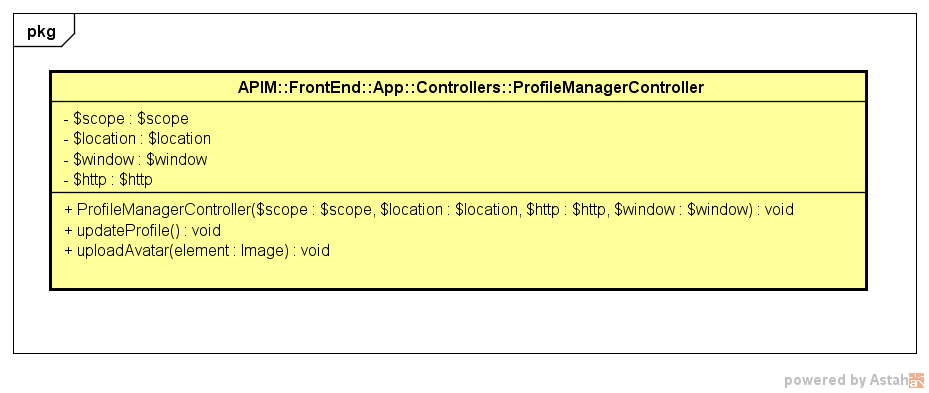
\includegraphics
	[width=0.7\linewidth]
	{images/APIM/FrontEnd/Controllers/ProfileManagerController.png}
	\caption{APIM::FrontEnd::App::Controllers::ProfileManagerController}
\end{figure}

\begin{itemize}
	\item \textbf{Descrizione:} ProfileManagerController permette di gestire il profilo personale di un
utente, fornendo le funzionalità all'utente per poter modificare i propri dati.
	\item \textbf{Attributi:}
		\begin{itemize}
		
			\item \textbf{\$scope : \$scope}\\
			Campo dati contenente un riferimento all'oggetto \$scope creato da AngularJS, viene utilizzato come mezzo di comunicazione tra il controller e la view. Contiene gli oggetti che definiscono il model dell'applicazione;
			
			\item \textbf{\$rootScope : \$rootScope}\\
			Campo dati contenente il riferimento all'oggetto globale \$rootScope creato da AngularJS. Viene utilizzato per rendere accessibile a tutti i controllers e a tutte le views l'oggetto UserDetailsModel;
				
			\item \textbf{\$timeout : \$timeout }\\
			Campo dati contenente il riferimento all'oggetto globale \$timeout creato da AngularJS. Il valore di ritorno di una chiamata alla funzione di \$timeout è una promise, la quale
sarà risolta quando avverrà il ritardo e la funzione di timeout eseguita;

			\item \textbf{\$http : \$http }\\
			Campo dati che contiene un riferimento al servizio \$http che permette la comunicazione con il protocollo HTTP;
				
			\item \textbf{user : UserDetailsModel }\\
			Campo dati che si riferisce alla classe che rappresenta il modello di un utente.
				
		\end{itemize}
	\item \textbf{Metodi:}
		\begin{itemize}
		
			\item \textbf{ProfileManagerController(\$scope : \$scope, \$rootScope : \$rootScope, user : UserDetailsModel) : void}\\
			Metodo costruttore della classe;
			\begin{description}
    			\item[\textbf{Parametri:}]
			\end{description}
			\begin{itemize}
				\item \textbf{\$scope : \$scope}\\
				Parametro che contiene un riferimento all'oggetto \$scope di AngularJS, impiegato nella comunicazione tra i rispettivi view e controller. Contiene gli oggetti che definiscono i model dell'applicazione;
				
				\item \textbf{\$rootScope : \$rootScope}\\
				Parametro che contiene il riferimento all'oggetto globale \$rootScope di AngularJS. Viene utilizzato per rendere accessibile a view e controller l'oggetto UserDetailsModel.
				
				\item \textbf{user: UserDetailsModel}\\
				Parametro che rappresenta un utente.
			\end{itemize}
			
			\item \textbf{confirm(user : Object, imageObject : Object) : void}\\
			Metodo per confermare le modifiche desiderate al proprio profilo. Per attuare le modifiche, si serve di un'operazione di un servizio esposto dal package \textbf{Services}.
			\begin{description}
    			\item[\textbf{Parametri:}]
			\end{description}
			\begin{itemize}
				\item \textbf{user}\\
				Parametro che rappresenta un utente;
				
				\item \textbf{imageObject}\\
				Parametro che rappresenta un file immagine.
			\end{itemize}
			
			\item \textbf{getUserDetails(email : string) : UserDetailsModel}\\
			Metodo per recuperare i propri dati personali. Si serve di un'operazione di un servizio esposto dal package \textbf{Services}.
			\begin{description}
    			\item[\textbf{Parametri:}]
			\end{description}
			\begin{itemize}
				\item \textbf{email}\\
				Parametro che rappresenta un indirizzo email.
			\end{itemize}
			
		\end{itemize}
	\item \textbf{Relazioni con altre classi:}
		\begin{itemize}
			\item Ricava i dati necessari dal package \textbf{Services};
			\item Gestisce il funzionamento della view \textbf{ProfileManager};
			\item Il model \textbf{UsersDetailModel} che contiene le informazioni per rappresentare un utente.
		\end{itemize}
\end{itemize}

\paragraph{APIM::FrontEnd::App::Controllers::APIRegistrationController}

\begin{figure}[H]
	\centering
	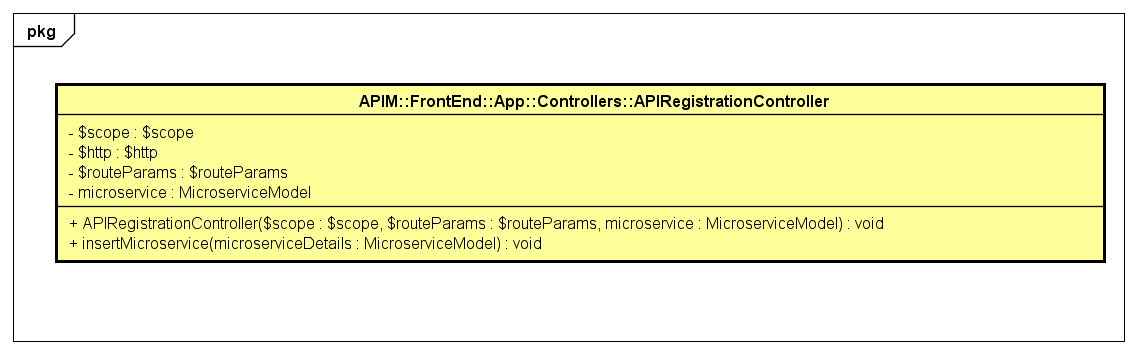
\includegraphics
	[width=0.7\linewidth]
	{images/APIM/FrontEnd/Controllers/APIRegistrationController.png}
	\caption{APIM::FrontEnd::App::Controllers::APIRegistrationController}
\end{figure}

\begin{itemize}
	\item \textbf{Descrizione:} APIRegistrationController permette di gestire l'inserimento di una API, fornendo tutte le funzionalità atte alla corretta esposizione di un microservizio di uno sviluppatore, utente della piattaforma API Market.
	\item \textbf{Attributi:}
		\begin{itemize}
		
			\item \textbf{\$scope : \$scope}\\
			Campo dati contenente un riferimento all'oggetto \$scope creato da AngularJS, viene utilizzato come mezzo di comunicazione tra il controller e la view. Contiene gli oggetti che definiscono il model dell'applicazione;
			
			\item \textbf{\$routeParams : \$routeParams}\\
			Parametro contenente il riferimento all'oggetto globale \$routeParams creato da AngularJS. Tale servizio permette di recuperare il set di variabili presenti nell'URL;

			\item \textbf{\$http : \$http }\\
			Campo dati che contiene un riferimento al servizio \$http che permette la comunicazione con il protocollo HTTP;
				
			\item \textbf{microservice : MicroserviceModel }\\
			Campo dati che si riferisce alla classe che rappresenta il modello di un microservizio.
				
		\end{itemize}
	\item \textbf{Metodi:}
		\begin{itemize}
		
			\item \textbf{APIRegistrationController(\$scope : \$scope, \$routeParams : \$routeParams, microservice : MicroserviceModel) : void}\\
			Metodo costruttore della classe.
			\begin{description}
    			\item[\textbf{Parametri:}]
			\end{description}
			\begin{itemize}
				\item \textbf{\$scope}\\
				Parametro che contiene un riferimento all'oggetto \$scope di AngularJS, impiegato nella comunicazione tra i rispettivi view e controller. Contiene gli oggetti che definiscono i model dell'applicazione;
				
				\item \textbf{\$routeParams}\\
				Parametro che contiene il riferimento all'oggetto globale \$routeParams di AngularJS. Permette di recuperare il set di variabili presenti nell'url;
				
				\item \textbf{microservice}\\
				Parametro che rappresenta un microservizio.
			\end{itemize}
			
			\item \textbf{insertMicroservice(microserviceDetails : MicroserviceModel) : void}\\
			Metodo per registrare un nuovo microservizio in API Market. Si serve di un'operazione di un servizio esposto dal package \textbf{Services}.
			\begin{description}
    			\item[\textbf{Parametri:}]
			\end{description}
			\begin{itemize}
				\item \textbf{microserviceDetails}\\
				Parametro che rappresenta un microservizio.
			\end{itemize}
			
		\end{itemize}
	\item \textbf{Relazioni con altre classi:}
		\begin{itemize}
			\item Ricava i dati necessari dal package \textbf{Services};
			\item Gestisce il funzionamento della view \textbf{RegisterAPI};
			\item Il model \textbf{MicroserviceModel} che contiene le informazioni per rappresentare un microservizio.
		\end{itemize}
\end{itemize}

\paragraph{APIM::FrontEnd::App::Controllers::SellingPolicyController}

\begin{figure}[H]
	\centering
	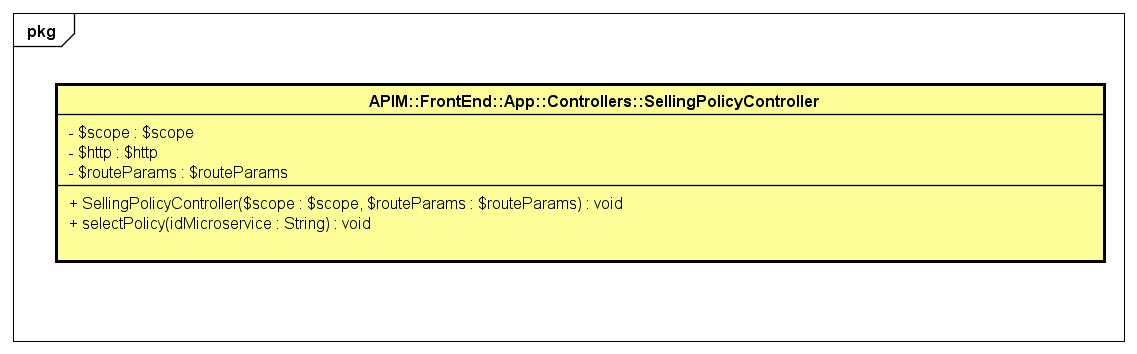
\includegraphics
	[width=0.7\linewidth]
	{images/APIM/FrontEnd/Controllers/SellingPolicyController.png}
	\caption{APIM::FrontEnd::App::Controllers::SellingPolicyController}
\end{figure}

\begin{itemize}
	\item \textbf{Descrizione:} SellingPolicyController permette di gestire le policy di vendita dei
microservizi.
	\item \textbf{Attributi:}
		\begin{itemize}
		
			\item \textbf{\$scope : \$scope}\\
			Campo dati contenente un riferimento all'oggetto \$scope creato da AngularJS, viene utilizzato come mezzo di comunicazione tra il controller e la view. Contiene gli oggetti che definiscono il model dell'applicazione;
			
			\item \textbf{\$routeParams : \$routeParams}\\
			Parametro contenente il riferimento all'oggetto globale \$routeParams creato da AngularJS. Tale servizio permette di recuperare il set di variabili presenti nell'URL;

			\item \textbf{\$http : \$http }\\
			Campo dati che contiene un riferimento al servizio \$http che permette la comunicazione con il protocollo HTTP.
				
		\end{itemize}
	\item \textbf{Metodi:}
		\begin{itemize}
		
			\item \textbf{SellingPolicyController(\$scope : \$scope, \$routeParams : \$routeParams) : void}\\
			Metodo costruttore della classe.
			\begin{description}
    			\item[\textbf{Parametri:}]
			\end{description}
			\begin{itemize}
				\item \textbf{\$scope}\\
				Parametro che contiene un riferimento all'oggetto \$scope di AngularJS, impiegato nella comunicazione tra i rispettivi view e controller. Contiene gli oggetti che definiscono i model dell'applicazione;
				
				\item \textbf{\$routeParams}\\
				Parametro che contiene il riferimento all'oggetto globale \$routeParams di AngularJS. Permette di recuperare il set di variabili presenti nell'url.
			\end{itemize}
			
			\item \textbf{selectPolicy(idMicroservice : string) : void}\\
			Metodo per selezionare una policy di vendita.
			\begin{description}
    			\item[\textbf{Parametri:}]
			\end{description}
			\begin{itemize}
				\item \textbf{idMicroservice}\\
				Parametro che contiene l'id di un microservizio.
			\end{itemize}
			
		\end{itemize}
	\item \textbf{Relazioni con altre classi:}
		\begin{itemize}
			\item Gestisce il funzionamento della view \textbf{SellingPolicy}.
		\end{itemize}
\end{itemize}

\paragraph{APIM::FrontEnd::App::Controllers::UserRegistrationController}

\begin{figure}[H]
	\centering
	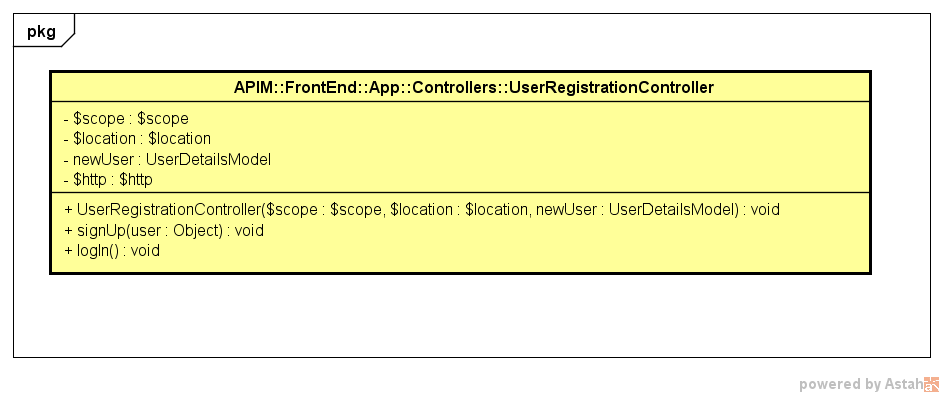
\includegraphics
	[width=0.7\linewidth]
	{images/APIM/FrontEnd/Controllers/UserRegistrationController.png}
	\caption{APIM::FrontEnd::App::Controllers::SignUpController}
\end{figure}

\begin{itemize}
	\item \textbf{Descrizione:} UserRegistrationController permette di gestire la registrazione di un
utente al sistema, fornendone le funzionalità preposte.
	\item \textbf{Attributi:}
		\begin{itemize}
		
			\item \textbf{\$scope : \$scope}\\
			Campo dati contenente un riferimento all'oggetto \$scope creato da AngularJS, viene utilizzato come mezzo di comunicazione tra il controller e la view. Contiene gli oggetti che definiscono il model dell'applicazione;
			
			\item \textbf{\$location : \$location}\\
			Campo dati contenente un riferimento al servizio creato da AngularJS che permette di accedere alla barra degli indirizzi del browser, i cambiamenti all'URL nella barra degli indirizzi si riflettono in questo oggetto e viceversa;

			\item \textbf{\$http : \$http }\\
			Campo dati che contiene un riferimento al servizio \$http che permette la comunicazione con il protocollo HTTP;
				
			\item \textbf{user : UserDetailsModel }\\
			Campo dati che si riferisce alla classe che rappresenta il modello di un utente.
				
		\end{itemize}
	\item \textbf{Metodi:}
		\begin{itemize}
		
			\item \textbf{UserRegistrationController(\$scope : \$scope, \$location : \$location, newUser : UserDetailsModel) : void}\\
			Metodo costruttore della classe;
			\begin{description}
    			\item[\textbf{Parametri:}]
			\end{description}
			\begin{itemize}
				\item \textbf{\$scope}\\
				Parametro che contiene un riferimento all'oggetto \$scope di AngularJS, impiegato nella comunicazione tra i rispettivi view e controller. Contiene gli oggetti che definiscono i model dell'applicazione;
				
				\item \textbf{\$location}\\
				Parametro che contiene un riferimento al servizio di AngularJS che permette di accedere alla barra degli indirizzi del browser, così da controllarne i cambiamenti;
				
				\item \textbf{newUser}\\
				Parametro che rappresenta un nuovo utente.
			\end{itemize}
			
			\item \textbf{signUp(user : Object) : void}\\
			Metodo per registrare un nuovo cliente in API Market. Si serve di un'operazione di un servizio esposto dal package \textbf{Services}.
			\begin{description}
    			\item[\textbf{Parametri:}]
			\end{description}
			\begin{itemize}
				\item \textbf{user}\\
				Parametro che rappresenta un utente.
			\end{itemize}
			
			\item \textbf{login() : void}\\
			Metodo per effettuare il login. Per controllare la validità dei dati immessi, si serve di un'operazione di un servizio esposto dal package \textbf{Services}.
			
		\end{itemize}
	\item \textbf{Relazioni con altre classi:}
		\begin{itemize}
			\item Ricava i dati necessari dal package \textbf{Services};
			\item Gestisce il funzionamento della view \textbf{RegisterUser};
			\item Il model \textbf{UsersDetailModel} che contiene le informazioni per rappresentare un utente.
		\end{itemize}
\end{itemize}

\paragraph{APIM::FrontEnd::App::Controllers::APIRegisteredController}

\begin{figure}[H]
	\centering
	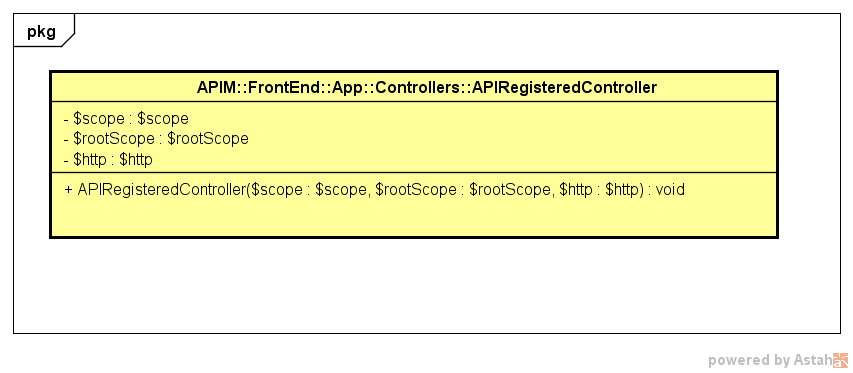
\includegraphics
	[width=0.7\linewidth]
	{images/APIM/FrontEnd/Controllers/APIRegisteredController.png}
	\caption{APIM::FrontEnd::App::Controllers::APIRegisteredController}
\end{figure}

\begin{itemize}
	\item \textbf{Descrizione:} APIRegisteredController permette di gestire le informazioni di una
API precedentemente inserita.
	\item \textbf{Attributi:}
		\begin{itemize}
		
			\item \textbf{\$scope : \$scope}\\
			Campo dati contenente un riferimento all'oggetto \$scope creato da AngularJS, viene utilizzato come mezzo di comunicazione tra il controller e la view. Contiene gli oggetti che definiscono il model dell'applicazione;
			
			\item \textbf{\$rootScope : \$rootScope}\\
			Campo dati contenente il riferimento all'oggetto globale \$rootScope creato da AngularJS. Viene utilizzato per rendere accessibile a tutti i controllers e a tutte le views l'oggetto MicroserviceModel;

			\item \textbf{\$http : \$http }\\
			Campo dati che contiene un riferimento al servizio \$http che permette la comunicazione con il protocollo HTTP;
				
			\item \textbf{microservice : MicroserviceModel }\\
			Campo dati che si riferisce alla classe che rappresenta il modello di un microservizio.
				
		\end{itemize}
	\item \textbf{Metodi:}
		\begin{itemize}
		
			\item \textbf{APIRegisteredController(\$scope : \$scope, \$rootScope : \$rootScope, microservice : MicroserviceModel) : void}\\
			Metodo costruttore della classe;
			\begin{description}
    			\item[\textbf{Parametri:}]
			\end{description}
			\begin{itemize}
				\item \textbf{\$scope}\\
				Parametro che contiene un riferimento all'oggetto \$scope di AngularJS, impiegato nella comunicazione tra i rispettivi view e controller. Contiene gli oggetti che definiscono i model dell'applicazione;
				
				\item \textbf{\$rootScope}\\
				Parametro che contiene il riferimento all'oggetto globale \$rootScope di AngularJS. Viene utilizzato per rendere accessibile a view e controller l'oggetto MicroserviceModel;
				
				\item \textbf{microservice}\\
				Parametro che rappresenta un microservizio.
			\end{itemize}
			
			\item \textbf{getMicroservicesDetails(email : string) : Array<MicroserviceModel>}\\
			Metodo per visualizzare le informazioni di un proprio microservizio registrato. Si serve di un'operazione di un servizio esposto dal package \textbf{Services};
			\begin{description}
    			\item[\textbf{Parametri:}]
			\end{description}
			\begin{itemize}
				\item \textbf{email}\\
				Parametro che rappresenta un indirizzo email.
			\end{itemize}
			
			\item \textbf{setMicroservice(newInfo : MicroserviceModel) : void}\\
			Metodo per modificare le informazioni di un proprio microservizio registrato. Si serve di un'operazione di un servizio esposto dal package \textbf{Services}.
			\begin{description}
    			\item[\textbf{Parametri:}]
			\end{description}
			\begin{itemize}
				\item \textbf{newInfo}\\
				Parametro che rappresenta un microservizio aggiornato.
			\end{itemize}

		\end{itemize}
	\item \textbf{Relazioni con altre classi:}
		\begin{itemize}
			\item Ricava i dati necessari dal package \textbf{Services};
			\item Gestisce il funzionamento della view \textbf{APIRegistered};
			\item Il model \textbf{MicroserviceModel} che contiene le informazioni per rappresentare un microservizio.
		\end{itemize}
\end{itemize}

\paragraph{APIM::FrontEnd::App::Controllers::SearchController}

\begin{figure}[H]
	\centering
	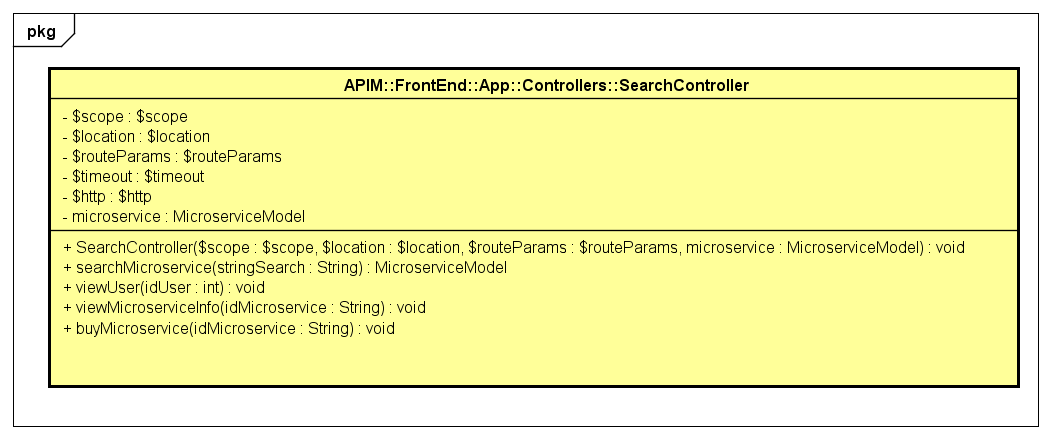
\includegraphics
	[width=0.7\linewidth]
	{images/APIM/FrontEnd/Controllers/SearchController.png}
	\caption{APIM::FrontEnd::App::Controllers::SearchController}
\end{figure}

\begin{itemize}
	\item \textbf{Descrizione:} SearchController permette di gestire la ricerca di microservizi all'interno
di API Market, fornendo all'utente le funzionalità di ricerca tramite
categorie e keywords per sviluppatori e microservizi.
	\item \textbf{Attributi:}
		\begin{itemize}
		
			\item \textbf{\$scope : \$scope}\\
			Campo dati contenente un riferimento all'oggetto \$scope creato da AngularJS, viene utilizzato come mezzo di comunicazione tra il controller e la view. Contiene gli oggetti che definiscono il model dell'applicazione;

			\item \textbf{\$routeParams : \$routeParams}\\
			Parametro contenente il riferimento all'oggetto globale \$routeParams creato da AngularJS. Tale servizio permette di recuperare il set di variabili presenti nell'URL.			
			
			\item \textbf{\$location : \$location}\\
			Campo dati contenente un riferimento al servizio creato da AngularJS che permette di accedere alla barra degli indirizzi del browser, i cambiamenti all'URL nella barra degli indirizzi si riflettono in questo oggetto e viceversa;
			
			\item \textbf{\$rootScope : \$rootScope}\\
			Campo dati contenente il riferimento all'oggetto globale \$rootScope creato da AngularJS. Viene utilizzato per rendere accessibile a tutti i controllers e a tutte le views l'oggetto MicroserviceModel;
			
			\item \textbf{\$timeout : \$timeout }\\
			Campo dati contenente il riferimento all'oggetto globale \$timeout creato da AngularJS. Il valore di ritorno di una chiamata alla funzione di \$timeout è una promise, la quale sarà risolta quando avverrà il ritardo e la funzione di timeout eseguita;

			\item \textbf{\$http : \$http }\\
			Campo dati che contiene un riferimento al servizio \$http che permette la comunicazione con il protocollo HTTP;
				
			\item \textbf{microservice : MicroserviceModel }\\
			Campo dati che si riferisce alla classe che rappresenta il modello di un microservizio.
				
		\end{itemize}
	\item \textbf{Metodi:}
		\begin{itemize}
		
			\item \textbf{SearchController(\$scope : \$scope, \$location : \$location, \$routeParams : \$routeParams, microservice : MicroserviceModel) : void}\\
			Metodo costruttore della classe;
			\begin{description}
    			\item[\textbf{Parametri:}]
			\end{description}
			\begin{itemize}
				\item \textbf{\$scope}\\
				Parametro che contiene un riferimento all'oggetto \$scope di AngularJS, impiegato nella comunicazione tra i rispettivi view e controller. Contiene gli oggetti che definiscono i model dell'applicazione;
				
				\item \textbf{\$location}\\
				Parametro che contiene un riferimento al servizio di AngularJS che permette di accedere alla barra degli indirizzi del browser, così da controllarne i cambiamenti;
				
				\item \textbf{\$routeParams}\\
				Parametro che contiene il riferimento all'oggetto globale \$routeParams di AngularJS. Permette di recuperare il set di variabili presenti nell'url;
				
				\item \textbf{microservice}\\
				Parametro che rappresenta un microservizio.
			\end{itemize}
			
			\item \textbf{searchMicroservice(stringSearch : string) : MicroserviceModel}\\
			Metodo per la ricerca della lista di API che corrispondono alle keywords immesse. Si serve di un'operazione di un servizio esposto dal package \textbf{Services}.
			\begin{description}
    			\item[\textbf{Parametri:}]
			\end{description}
			\begin{itemize}
				\item \textbf{stringSearch}\\
				Parametro che rappresenta una stringa di keywords di ricerca.
			\end{itemize}
			
			\item \textbf{viewUser(idUser : int) : void}\\
			Metodo per visualizzare la pagina dell'utente di una specifica API. Si serve di un'operazione di un servizio esposto dal package \textbf{Services}.
			\begin{description}
    			\item[\textbf{Parametri:}]
			\end{description}
			\begin{itemize}
				\item \textbf{idUser}\\
				Parametro che rappresenta l'id di un utente da visualizzare.
			\end{itemize}
			
			\item \textbf{viewMicroserviceInfo(idMicroservice : string) : void}\\
			Metodo per visualizzare la pagina dell'API di una specifica API della lista dei risultati della ricerca. Si serve di un'operazione di un servizio esposto dal package \textbf{Services}.
			\begin{description}
    			\item[\textbf{Parametri:}]
			\end{description}
			\begin{itemize}
				\item \textbf{idMicroservice}\\
				Parametro che rappresenta l'id di un microservizio da visualizzare.
			\end{itemize}
			
			\item \textbf{buyMicroservice(idMicroservice : string) : void}\\
			Metodo per iniziare l'acquisto di una specifica API. Si serve della procedura di acquisto di PayPal.
			\begin{description}
    			\item[\textbf{Parametri:}]
			\end{description}
			\begin{itemize}
				\item \textbf{idMicroservice}\\
				Parametro che rappresenta l'id di un microservizio da acquistare.
			\end{itemize}
			
		\end{itemize}
	\item \textbf{Relazioni con altre classi:}
		\begin{itemize}
			\item Ricava i dati necessari dal package \textbf{Services};
			\item Gestisce il funzionamento della view \textbf{API};
			\item Il model \textbf{MicroserviceModel} che contiene le informazioni per rappresentare un microservizio.
		\end{itemize}
\end{itemize}

\paragraph{APIM::FrontEnd::App::Controllers::TransactionsListController}

\begin{figure}[H]
	\centering
	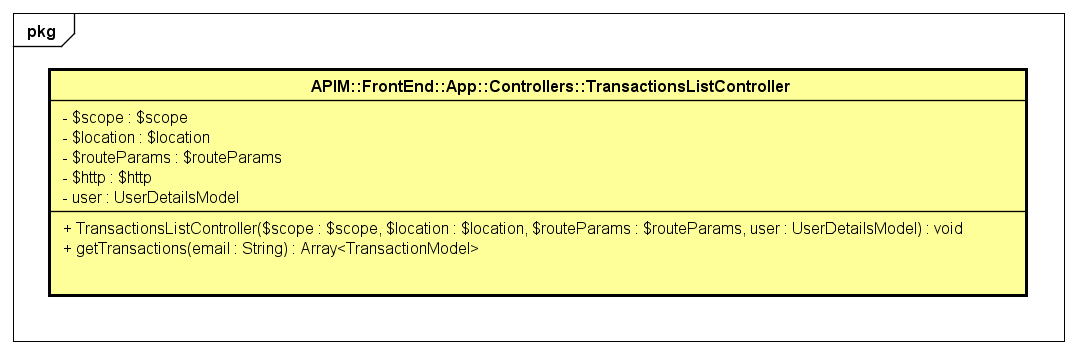
\includegraphics
	[width=0.7\linewidth]
	{images/APIM/FrontEnd/Controllers/TransactionsListController.png}
	\caption{APIM::FrontEnd::App::Controllers::TransactionsListController}
\end{figure}

\begin{itemize}
	\item \textbf{Descrizione:} TransactionsListController permette di gestire lo storico delle transazioni
di un utente di API Market.
	\item \textbf{Attributi:}
		\begin{itemize}
		
			\item \textbf{\$scope : \$scope}\\
			Campo dati contenente un riferimento all'oggetto \$scope creato da AngularJS, viene utilizzato come mezzo di comunicazione tra il controller e la view. Contiene gli oggetti che definiscono il model dell'applicazione;

			\item \textbf{\$routeParams : \$routeParams}\\
			Parametro contenente il riferimento all'oggetto globale \$routeParams creato da AngularJS. Tale servizio permette di recuperare il set di variabili presenti nell'URL.			
			
			\item \textbf{\$location : \$location}\\
			Campo dati contenente un riferimento al servizio creato da AngularJS che permette di accedere alla barra degli indirizzi del browser, i cambiamenti all'URL nella barra degli indirizzi si riflettono in questo oggetto e viceversa;
			
			\item \textbf{\$rootScope : \$rootScope}\\
			Campo dati contenente il riferimento all'oggetto globale \$rootScope creato da AngularJS. Viene utilizzato per rendere accessibile a tutti i controllers e a tutte le views l'oggetto TransactionModel;

			\item \textbf{\$http : \$http }\\
			Campo dati che contiene un riferimento al servizio \$http che permette la comunicazione con il protocollo HTTP;
				
			\item \textbf{transaction : TransactionModel }\\
			Campo dati che si riferisce alla classe che rappresenta il modello di una transazione.
				
		\end{itemize}
	\item \textbf{Metodi:}
		\begin{itemize}
		
			\item \textbf{TransactionsListController(\$scope : \$scope, \$location : \$location, \$routeParams : \$routeParams, user : UserDetailsModel) : void}\\
			Metodo costruttore della classe;
			\begin{description}
    			\item[\textbf{Parametri:}]
			\end{description}
			\begin{itemize}
				\item \textbf{\$scope}\\
				Parametro che contiene un riferimento all'oggetto \$scope di AngularJS, impiegato nella comunicazione tra i rispettivi view e controller. Contiene gli oggetti che definiscono i model dell'applicazione;
				\item \textbf{\$location}\\
				Parametro che contiene un riferimento al servizio di AngularJS che permette di accedere alla barra degli indirizzi del browser, così da controllarne i cambiamenti;
			
				\item \textbf{\$routeParams}\\
				Parametro che contiene il riferimento all'oggetto globale \$routeParams di AngularJS. Permette di recuperare il set di variabili presenti nell'url;
				
				\item \textbf{user}\\
				Parametro che rappresenta un utente.
			\end{itemize}
			
			\item \textbf{getTransactions(email : string) : Array<TransactionModel>}\\
			Metodo per visualizzare la lista delle transazioni di un utente. Si serve di un'operazione di un servizio esposto dal package \textbf{Services}.
			\begin{description}
    			\item[\textbf{Parametri:}]
			\end{description}
			\begin{itemize}
				\item \textbf{email}\\
				Parametro che contiene un indirizzo email.
			\end{itemize}
			
		\end{itemize}
	\item \textbf{Relazioni con altre classi:}
		\begin{itemize}
			\item Ricava i dati necessari dal package \textbf{Services};
			\item Gestisce il funzionamento della view \textbf{TransactionsList};
			\item Il model \textbf{UserDetailsModel} che contiene le informazioni per rappresentare un utente.
			\item Il model \textbf{TransactionModel} che contiene le informazioni per rappresentare una transazione.
		\end{itemize}
\end{itemize}

\paragraph{APIM::FrontEnd::App::Controllers::AdminManagerController}

\begin{figure}[H]
	\centering
	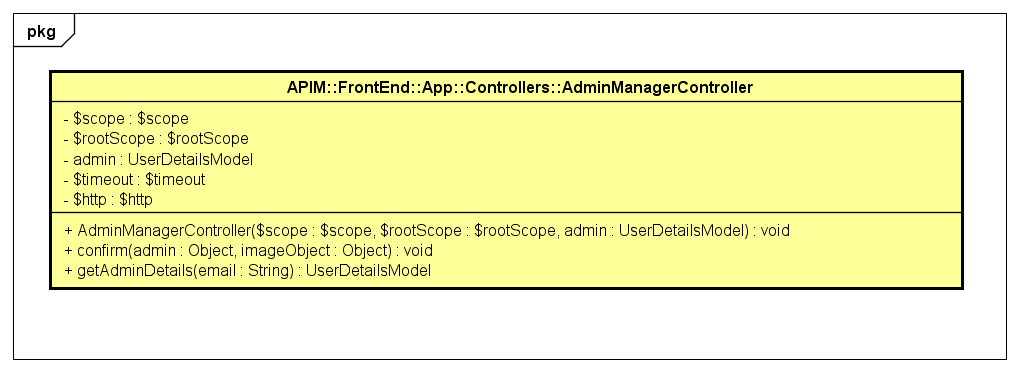
\includegraphics
	[width=0.7\linewidth]
	{images/APIM/FrontEnd/Controllers/AdminManagerController.png}
	\caption{APIM::FrontEnd::App::Controllers::AdminManagerController}
\end{figure}

\begin{itemize}
	\item \textbf{Descrizione:} AdminManagerController permette di gestire il profilo di un amministratore della piattaforma API Market, fornendo le funzionalità per poter modificare i propri dati e moderare utenti ed API.
	\item \textbf{Attributi:}
		\begin{itemize}
		
			\item \textbf{\$scope : \$scope}\\
			Campo dati contenente un riferimento all'oggetto \$scope creato da AngularJS, viene utilizzato come mezzo di comunicazione tra il controller e la view. Contiene gli oggetti che definiscono il model dell'applicazione;
			
			\item \textbf{\$rootScope : \$rootScope}\\
			Campo dati contenente il riferimento all'oggetto globale \$rootScope creato da AngularJS. Viene utilizzato per rendere accessibile a tutti i controllers e a tutte le views l'oggetto UserDetailsModel;
			
			\item \textbf{\$timeout : \$timeout }\\
			Campo dati contenente il riferimento all'oggetto globale \$timeout creato da AngularJS. Il valore di ritorno di una chiamata alla funzione di \$timeout è una promise, la quale sarà risolta quando avverrà il ritardo e la funzione di timeout eseguita;

			\item \textbf{\$http : \$http }\\
			Campo dati che contiene un riferimento al servizio \$http che permette la comunicazione con il protocollo HTTP;
				
			\item \textbf{admin : UserDetailsModel }\\
			Campo dati che si riferisce alla classe che rappresenta il modello di un utente.
				
		\end{itemize}
	\item \textbf{Metodi:}
		\begin{itemize}
		
			\item \textbf{AdminManagerController(\$scope : \$scope, \$rootScope : \$rootScope, admin : UserDetailsModel) : void}\\
			Metodo costruttore della classe.
			\begin{description}
    			\item[\textbf{Parametri:}]
			\end{description}
			\begin{itemize}
				\item \textbf{\$scope}\\
				Parametro che contiene un riferimento all'oggetto \$scope di AngularJS, impiegato nella comunicazione tra i rispettivi view e controller. Contiene gli oggetti che definiscono i model dell'applicazione;
				
				\item \textbf{\$rootScope}\\
				Parametro che contiene il riferimento all'oggetto globale \$rootScope di AngularJS. Viene utilizzato per rendere accessibile a view e controller l'oggetto UserDetailsModel;
				
				\item \textbf{admin}\\
				Parametro che rappresenta un admin.
			\end{itemize}
			
			\item \textbf{confirm(admin : Object, imageObject : Object) : void}\\
			Metodo per confermare le modifiche desiderate al profilo admin. Si serve di un'operazione di un servizio esposto dal package \textbf{Services};
			\begin{description}
    			\item[\textbf{Parametri:}]
			\end{description}
			\begin{itemize}
				\item \textbf{admin}\\
				Parametro che rappresenta un admin;
				
				\item \textbf{imageObject}\\
				Parametro che rappresenta un file immagine.
			\end{itemize}
			
			\item \textbf{getAdminDetails(email : string) : UserDetailsModel}\\
			Metodo per visualizzare le informazioni personali del profilo admin. Si serve di un'operazione di un servizio esposto dal package \textbf{Services}.
			\begin{description}
    			\item[\textbf{Parametri:}]
			\end{description}
			\begin{itemize}
				\item \textbf{email}\\
				Parametro che rappresenta un indirizzo email;
			\end{itemize}
			
		\end{itemize}
	\item \textbf{Relazioni con altre classi:}
		\begin{itemize}
			\item Ricava i dati necessari dal package \textbf{Services};
			\item Gestisce il funzionamento della view \textbf{AdminManager};
			\item Il model \textbf{UsersDetailModel} che contiene le informazioni per rappresentare un utente.
		\end{itemize}
\end{itemize}

\paragraph{APIM::FrontEnd::App::Controllers::AdminModerationController}

\begin{figure}[H]
	\centering
	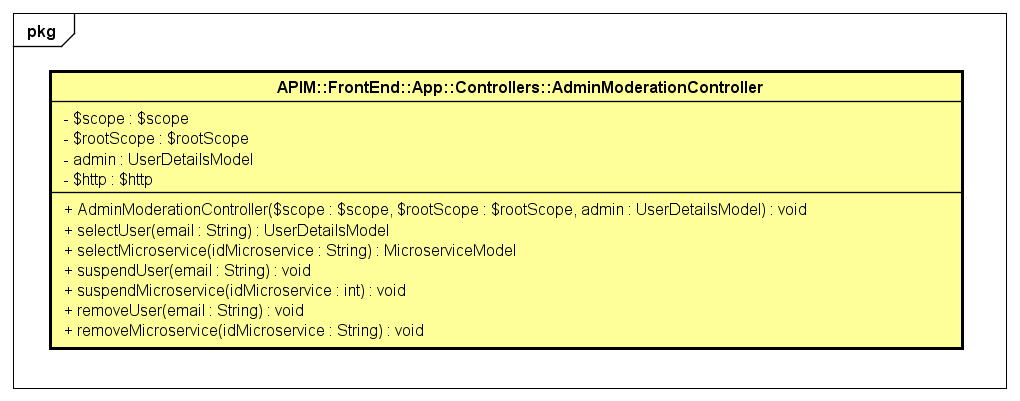
\includegraphics
	[width=0.7\linewidth]
	{images/APIM/FrontEnd/Controllers/AdminModerationController.png}
	\caption{APIM::FrontEnd::App::Controllers::AdminModerationController}
\end{figure}

\begin{itemize}
	\item \textbf{Descrizione:} AdminModerationController permette di gestire la moderazione di
un utente (cliente o sviluppatore che sia) e di API, fornendo le funzionalità per la
sospensione e rimozione.
	\item \textbf{Attributi:}
		\begin{itemize}
		
			\item \textbf{\$scope : \$scope}\\
			Campo dati contenente un riferimento all'oggetto \$scope creato da AngularJS, viene utilizzato come mezzo di comunicazione tra il controller e la view. Contiene gli oggetti che definiscono il model dell'applicazione;
			
			\item \textbf{\$rootScope : \$rootScope}\\
			Campo dati contenente il riferimento all'oggetto globale \$rootScope creato da AngularJS. Viene utilizzato per rendere accessibile a tutti i controllers e a tutte le views gli oggetti UserDetailsModel e MicroserviceModel;

			\item \textbf{\$http : \$http }\\
			Campo dati che contiene un riferimento al servizio \$http che permette la comunicazione con il protocollo HTTP;
				
			\item \textbf{admin : UserDetailsModel }\\
			Campo dati che si riferisce alla classe che rappresenta il modello di un utente.
			
			\item \textbf{microservice : MicroserviceModel }\\
			Campo dati che si riferisce alla classe che rappresenta il modello di un microservizio.
				
		\end{itemize}
	\item \textbf{Metodi:}
		\begin{itemize}
		
			\item \textbf{AdminManagerController(\$scope : \$scope, \$rootScope : \$rootScope, admin : UserDetailsModel) : void}\\
			Metodo costruttore della classe.
			\begin{description}
    			\item[\textbf{Parametri:}]
			\end{description}
			\begin{itemize}
				\item \textbf{\$scope}\\
				Parametro che contiene un riferimento all'oggetto \$scope di AngularJS, impiegato nella comunicazione tra i rispettivi view e controller. Contiene gli oggetti che definiscono i model dell'applicazione;
				
				\item \textbf{\$rootScope}\\
				Parametro che contiene il riferimento all'oggetto globale \$rootScope di AngularJS. Viene utilizzato per rendere accessibile a view e controller l'oggetto UserDetailsModel;
				
				\item \textbf{admin}\\
				Parametro che rappresenta un admin.
			\end{itemize}
			
			\item \textbf{selectUser(email : string) : UserDetailsModel}\\
			Metodo per selezionare un utente da moderare.
			\begin{description}
    			\item[\textbf{Parametri:}]
			\end{description}
			\begin{itemize}
				\item \textbf{email}\\
				Parametro che rappresenta un indirizzo email.
			\end{itemize}
			
			\item \textbf{selectMicroservice(idMicroservice : string) : MicroserviceModel}\\
			Metodo per selezionare una API da moderare.
			\begin{description}
    			\item[\textbf{Parametri:}]
			\end{description}
			\begin{itemize}
				\item \textbf{idMicroservice}\\
				Parametro che rappresenta l'id di un microservizio.
			\end{itemize}
			
			\item \textbf{suspendUser(email : string) : void}\\
			Metodo per sospendere l'utente selezionato. Si serve di un'operazione di un servizio esposto dal package \textbf{Services}.
			\begin{description}
    			\item[\textbf{Parametri:}]
			\end{description}
			\begin{itemize}
				\item \textbf{email}\\
				Parametro che rappresenta un indirizzo email.
			\end{itemize}
			
			\item \textbf{suspendMicroservice(idMicroservice : int) : void}\\
			Metodo per sospendere l'API selezionata. Si serve di un'operazione di un servizio esposto dal package \textbf{Services}.
			\begin{description}
    			\item[\textbf{Parametri:}]
			\end{description}
			\begin{itemize}
				\item \textbf{idMicroservice}\\
				Parametro che rappresenta l'id di un microservizio.
			\end{itemize}
			
			\item \textbf{removeUser(email : string) : void}\\
			Metodo per cancellare l'utente selezionato. Si serve di un'operazione di un servizio esposto dal package \textbf{Services}.
			\begin{description}
    			\item[\textbf{Parametri:}]
			\end{description}
			\begin{itemize}
				\item \textbf{email}\\
				Parametro che rappresenta un indirizzo email.
			\end{itemize}
			
			\item \textbf{removeMicroservice(idMicroservice : string) : void}\\
			Metodo per disabilitare il microservizio selezionato. Si serve di un'operazione di un servizio esposto dal package \textbf{Services}.
			\begin{description}
    			\item[\textbf{Parametri:}]
			\end{description}
			\begin{itemize}
				\item \textbf{idMicroservice}\\
				Parametro che rappresenta l'id di un microservizio.
			\end{itemize}
			
		\end{itemize}
	\item \textbf{Relazioni con altre classi:}
		\begin{itemize}
			\item Ricava i dati necessari dal package \textbf{Services};
			\item Gestisce il funzionamento della view \textbf{AdminModeration};
			\item Il model \textbf{UsersDetailModel} che contiene le informazioni per rappresentare un utente;
			\item Il model \textbf{MicroserviceModel} che contiene le informazioni per rappresentare un microservizio.
	\end{itemize}
\end{itemize}

\paragraph{APIM::FrontEnd::App::Controllers::LoginController}

\begin{figure}[H]
	\centering
	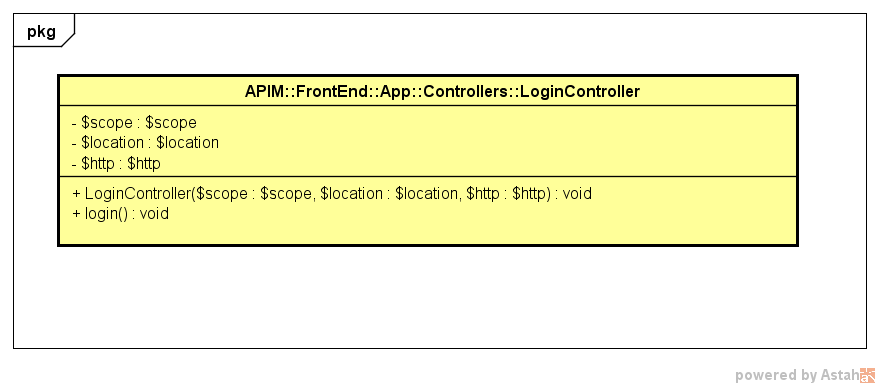
\includegraphics
	[width=0.7\linewidth]
	{images/APIM/FrontEnd/Controllers/LoginController.png}
	\caption{APIM::FrontEnd::App::Controllers::LoginController}
\end{figure}

\begin{itemize}
	\item \textbf{Descrizione:} LoginController permette di gestire il login di un utente alla piattaforma
API Market, fornendo le funzionalità di autenticazione al sistema, compresa la gestione di situazioni di errore di autenticazione.
	\item \textbf{Attributi:}
		\begin{itemize}
		
			\item \textbf{\$scope : \$scope}\\
			Campo dati contenente un riferimento all'oggetto \$scope creato da AngularJS, viene utilizzato come mezzo di comunicazione tra il controller e la view. Contiene gli oggetti che definiscono il model dell'applicazione;
			
			\item \textbf{\$rootScope : \$rootScope}\\
			Campo dati contenente il riferimento all'oggetto globale \$rootScope creato da AngularJS. Viene utilizzato per rendere accessibile a tutti i controllers e a tutte le views l'oggetto UserDetailsModel;
			
			\item \textbf{\$location : \$location}\\
			Campo dati contenente un riferimento al servizio creato da AngularJS che permette di accedere alla barra degli indirizzi del browser, i cambiamenti all'URL nella barra degli indirizzi si riflettono in questo oggetto e viceversa;

			\item \textbf{\$http : \$http }\\
			Campo dati che contiene un riferimento al servizio \$http che permette la comunicazione con il protocollo HTTP;
				
			\item \textbf{newUser : UserDetailsModel }\\
			Campo dati che si riferisce alla classe che rappresenta il modello di un utente.
				
		\end{itemize}
	\item \textbf{Metodi:}
		\begin{itemize}
		
			\item \textbf{LoginController(\$scope : \$scope, \$rootScope : \$rootScope, \$location : \$location, user : UserDetailsModel) : void}\\
			Metodo costruttore della classe.
			\begin{description}
    			\item[\textbf{Parametri:}]
			\end{description}
			\begin{itemize}
				\item \textbf{\$scope}\\
				Parametro che contiene un riferimento all'oggetto \$scope di AngularJS, impiegato nella comunicazione tra i rispettivi view e controller. Contiene gli oggetti che definiscono i model dell'applicazione;
				
				\item \textbf{\$rootScope}\\
				Parametro che contiene il riferimento all'oggetto globale \$rootScope di AngularJS. Viene utilizzato per rendere accessibile a view e controller l'oggetto UserDetailsModel;
				
				\item \textbf{\$location}\\
				Parametro che contiene un riferimento al servizio di AngularJS che permette di accedere alla barra degli indirizzi del browser, così da controllarne i cambiamenti;
				
				\item \textbf{user}\\
				Parametro che rappresenta un utente.
			\end{itemize}
			
			\item \textbf{logIn(email : string, password : string) : void}\\
			Metodo per effettuare il login. Per verificare la validità dei dati immessi, si serve di un'operazione di un servizio esposto dal package \textbf{Services}.
			\begin{description}
    			\item[\textbf{Parametri:}]
			\end{description}
			\begin{itemize}
				\item \textbf{email}\\
				Parametro che rappresenta un indirizzo email;
				
				\item \textbf{password}\\
				Parametro che rappresenta una password.
			\end{itemize}
			
			\item \textbf{registration() : void}\\
			Metodo per registrare un nuovo account utente. Si serve di un'operazione di un servizio esposto dal package \textbf{Services}.
			
			\item \textbf{recoveryPassword() : void}\\
			Metodo per recuperare la password di un utente. Per verificare l'esistenza dell'utente sbadato e per aggiornarne la password, si serve delle operazioni dei servizi esposti dal package \textbf{Services}.
			
		\end{itemize}
	\item \textbf{Relazioni con altre classi:}
		\begin{itemize}
			\item Ricava i dati necessari dal package \textbf{Services};
			\item Gestisce il funzionamento della view \textbf{Login};
			\item Il model \textbf{UsersDetailModel} che contiene le informazioni per rappresentare un utente.
		\end{itemize}
\end{itemize}

\paragraph{APIM::FrontEnd::App::Controllers::VirtualAccountController}

\begin{figure}[H]
	\centering
	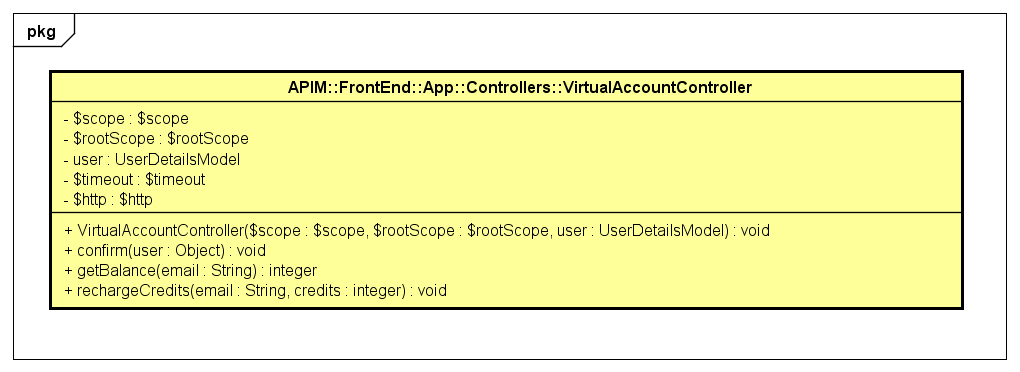
\includegraphics
	[width=0.7\linewidth]
	{images/APIM/FrontEnd/Controllers/VirtualAccountController.png}
	\caption{APIM::Front-End::App::Controllers::VirtualAccountController}
\end{figure}

\begin{itemize}
	\item \textbf{Descrizione:} VirtualAccountController permette di gestire il conto virtuale associato
al profilo di un utente, fornendo le funzionalità per la ricarica del saldo tramite PayPal.
	\item \textbf{Attributi:}
		\begin{itemize}
		
			\item \textbf{\$scope : \$scope}\\
			Campo dati contenente un riferimento all'oggetto \$scope creato da AngularJS, viene utilizzato come mezzo di comunicazione tra il controller e la view. Contiene gli oggetti che definiscono il model dell'applicazione;
			
			\item \textbf{\$rootScope : \$rootScope}\\
			Campo dati contenente il riferimento all'oggetto globale \$rootScope creato da AngularJS. Viene utilizzato per rendere accessibile a tutti i controllers e a tutte le views gli oggetti UserDetailsModel e TransactionModel;
			
			\item \textbf{\$location : \$location}\\
			Campo dati contenente un riferimento al servizio creato da AngularJS che permette di accedere alla barra degli indirizzi del browser, i cambiamenti all'URL nella barra degli indirizzi si riflettono in questo oggetto e viceversa;

			\item \textbf{\$http : \$http }\\
			Campo dati che contiene un riferimento al servizio \$http che permette la comunicazione con il protocollo HTTP;
				
			\item \textbf{user : UserDetailsModel }\\
			Campo dati che si riferisce alla classe che rappresenta il modello di un utente.
			
			\item \textbf{transaction : TransactionModel }\\
			Campo dati che si riferisce alla classe che rappresenta il modello di una transazione.
				
		\end{itemize}
	\item \textbf{Metodi:}
		\begin{itemize}
		
			\item \textbf{VirtualAccountController(\$scope : \$scope, \$rootScope : \$rootScope, user : UserDetailsModel) : void}\\
			Metodo costruttore della classe.
			\begin{description}
    			\item[\textbf{Parametri:}]
			\end{description}
			\begin{itemize}
				\item \textbf{\$scope}\\
				Parametro che contiene un riferimento all'oggetto \$scope di AngularJS, impiegato nella comunicazione tra i rispettivi view e controller. Contiene gli oggetti che definiscono i model dell'applicazione;
				
				\item \textbf{\$rootScope}\\
				Parametro che contiene il riferimento all'oggetto globale \$rootScope di AngularJS. Viene utilizzato per rendere accessibile a view e controller l'oggetto UserDetailsModel;
				
				\item \textbf{user}\\
				Parametro che rappresenta un utente.
			\end{itemize}
			
			\item \textbf{confirm(user : Object) : void}\\
			Metodo per confermare la ricarica dei crediti del conto virtuale dell'utente. Si serve di un'operazione di un servizio esposto dal package \textbf{Services}.
			\begin{description}
    			\item[\textbf{Parametri:}]
			\end{description}
			\begin{itemize}
				\item \textbf{user}\\
				Parametro che rappresenta un utente.
			\end{itemize}
			
			\item \textbf{getBalance(email : string) : int}\\
			Metodo per visualizzare il saldo attuale dei crediti dell'utente. Si serve di un'operazione di un servizio esposto dal package \textbf{Services}.
			\begin{description}
    			\item[\textbf{Parametri:}]
			\end{description}
			\begin{itemize}
				\item \textbf{email}\\
				Parametro che rappresenta un indirizzo email.
			\end{itemize}
			
			\item \textbf{rechargeCredits(email : string, credits : int) : void}\\
			Metodo per ricaricare i crediti del conto virtuale dell'utente. Si serve di un'operazione di un servizio esposto dal package \textbf{Services}.
			\begin{description}
    			\item[\textbf{Parametri:}]
			\end{description}
			\begin{itemize}
				\item \textbf{email}\\
				Parametro che rappresenta un indirizzo email;
				
				\item \textbf{credits}\\
				Parametro che rappresenta il numbero di crediti da acquistare;
			\end{itemize}
			
		\end{itemize}
	\item \textbf{Relazioni con altre classi:}
		\begin{itemize}
			\item Ricava i dati necessari dal package \textbf{Services};
			\item Gestisce il funzionamento della view \textbf{VirtualAccount};
			\item Il model \textbf{UsersDetailModel} che contiene le informazioni per rappresentare un utente.
		\end{itemize}
\end{itemize}

\paragraph{APIM::FrontEnd::App::Controllers::PasswordRecoveryController}

\begin{figure}[H]
	\centering
	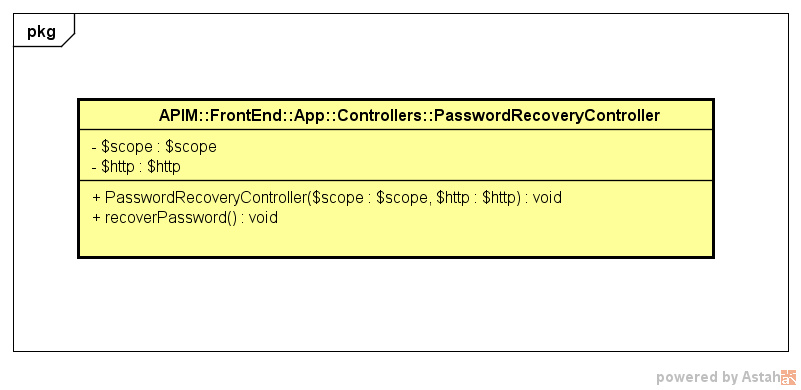
\includegraphics
	[width=0.7\linewidth]
	{images/APIM/FrontEnd/Controllers/PasswordRecoveryController.png}
	\caption{APIM::FrontEnd::App::Controllers::PasswordRecoveryController}
\end{figure}

\begin{itemize}
	\item \textbf{Descrizione:} PasswordRecoveryController permette di gestire il ripristino della password
dimenticata da un utente, fornendo tutte le funzionalità per il recupero della password dopo aver verificato l'identità dell'utente.
	\item \textbf{Attributi:}
		\begin{itemize}
		
			\item \textbf{\$scope : \$scope}\\
			Campo dati contenente un riferimento all'oggetto \$scope creato da AngularJS, viene utilizzato come mezzo di comunicazione tra il controller e la view. Contiene gli oggetti che definiscono il model dell'applicazione;
			
			\item \textbf{\$rootScope : \$rootScope}\\
			Campo dati contenente il riferimento all'oggetto globale \$rootScope creato da AngularJS. Viene utilizzato per rendere accessibile a tutti i controllers e a tutte le views l'oggetto UserDetailsModel;
			
			\item \textbf{\$location : \$location}\\
			Campo dati contenente un riferimento al servizio creato da AngularJS che permette di accedere alla barra degli indirizzi del browser, i cambiamenti all'URL nella barra degli indirizzi si riflettono in questo oggetto e viceversa;

			\item \textbf{\$http : \$http }\\
			Campo dati che contiene un riferimento al servizio \$http che permette la comunicazione con il protocollo HTTP;
				
			\item \textbf{user : UserDetailsModel }\\
			Campo dati che si riferisce alla classe che rappresenta il modello di un utente.

		\end{itemize}
	\item \textbf{Metodi:}
		\begin{itemize}
		
			\item \textbf{PasswordRecoveryController(\$scope : \$scope, \$location : \$location) : void}\\
			Metodo costruttore della classe.
			\begin{description}
    			\item[\textbf{Parametri:}]
			\end{description}
			\begin{itemize}
				\item \textbf{\$scope}\\
				Parametro che contiene un riferimento all'oggetto \$scope di AngularJS, impiegato nella comunicazione tra i rispettivi view e controller. Contiene gli oggetti che definiscono i model dell'applicazione;
				
				\item \textbf{\$location}\\
				Parametro che contiene un riferimento al servizio di AngularJS che permette di accedere alla barra degli indirizzi del browser, così da controllarne i cambiamenti.
				
			\end{itemize}
			
			\item \textbf{passwordForgot() : void}\\
			Metodo per recuperare la password dell'utente. Per aggiornare la nuova password, si serve di un'operazione di un servizio esposto dal package \textbf{Services}.
			
		\end{itemize}
	\item \textbf{Relazioni con altre classi:}
		\begin{itemize}
			\item Ricava i dati necessari dal package \textbf{Services};
			\item Gestisce il funzionamento della view \textbf{PasswordRecovery}.
		\end{itemize}
\end{itemize}

\paragraph{APIM::FrontEnd::App::Controllers::ResetPasswordController}

\begin{figure}[H]
	\centering
	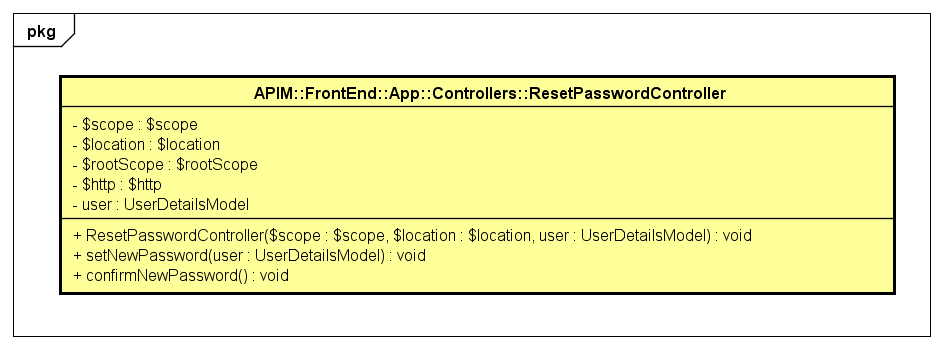
\includegraphics
	[width=0.7\linewidth]
	{images/APIM/FrontEnd/Controllers/ResetPasswordController.png}
	\caption{APIM::FrontEnd::App::Controllers::ResetPasswordController}
\end{figure}

\begin{itemize}
	\item \textbf{Descrizione:} ResetPasswordController permette di gestire il cambio password di un
utente autenticato al sistema, fornendo le funzionalità per il salvataggio di una nuova password.
	\item \textbf{Attributi:}
		\begin{itemize}
		
			\item \textbf{\$scope : \$scope}\\
			Campo dati contenente un riferimento all'oggetto \$scope creato da AngularJS, viene utilizzato come mezzo di comunicazione tra il controller e la view. Contiene gli oggetti che definiscono il model dell'applicazione;
			
			\item \textbf{\$rootScope : \$rootScope}\\
			Campo dati contenente il riferimento all'oggetto globale \$rootScope creato da AngularJS. Viene utilizzato per rendere accessibile a tutti i controllers e a tutte le views l'oggetto UserDetailsModel;
			
			\item \textbf{\$location : \$location}\\
			Campo dati contenente un riferimento al servizio creato da AngularJS che permette di accedere alla barra degli indirizzi del browser, i cambiamenti all'URL nella barra degli indirizzi si riflettono in questo oggetto e viceversa;

			\item \textbf{\$http : \$http }\\
			Campo dati che contiene un riferimento al servizio \$http che permette la comunicazione con il protocollo HTTP;
				
			\item \textbf{user : UserDetailsModel }\\
			Campo dati che si riferisce alla classe che rappresenta il modello di un utente.
				
		\end{itemize}
	\item \textbf{Metodi:}
		\begin{itemize}
		
			\item \textbf{ResetPasswordController(\$scope : \$scope, \$location : \$location, user : UserDetailsModel) : void) : void}\\
			Metodo costruttore della classe.
			\begin{description}
    			\item[\textbf{Parametri:}]
			\end{description}
			\begin{itemize}
				\item \textbf{\$scope}\\
				Parametro che contiene un riferimento all'oggetto \$scope di AngularJS, impiegato nella comunicazione tra i rispettivi view e controller. Contiene gli oggetti che definiscono i model dell'applicazione;
				
				\item \textbf{\$location}\\
				Parametro che contiene un riferimento al servizio di AngularJS che permette di accedere alla barra degli indirizzi del browser, così da controllarne i cambiamenti;
				
				\item \textbf{user}\\
				Parametro che rappresenta un utente.
			\end{itemize}
			
			\item \textbf{setNewPassword(user : UserDetailsModel) : void}\\
			Metodo per scegliere ed impostare una nuova password. Per aggiornare la nuova password, si serve di un'operazione di un servizio esposto dal package \textbf{Services}.
			\begin{description}
    			\item[\textbf{Parametri:}]
			\end{description}
			\begin{itemize}
				\item \textbf{user}\\
				Parametro che rappresenta un utente.
			\end{itemize}
			
			\item \textbf{ confirmNewPassword() : void}\\
			Metodo per confermare la nuova password. Si serve di un'operazione di un servizio esposto dal package \textbf{Services}.
			
		\end{itemize}
	\item \textbf{Relazioni con altre classi:}
		\begin{itemize}
			\item Ricava i dati necessari dal package \textbf{Services};
			\item Gestisce il funzionamento della view \textbf{ResetPassword};
			\item Il model \textbf{UsersDetailModel} che contiene le informazioni per rappresentare un utente.
		\end{itemize}
\end{itemize}

\paragraph{APIM::FrontEnd::App::Controllers::APIPurchasedController}

\begin{figure}[H]
	\centering
	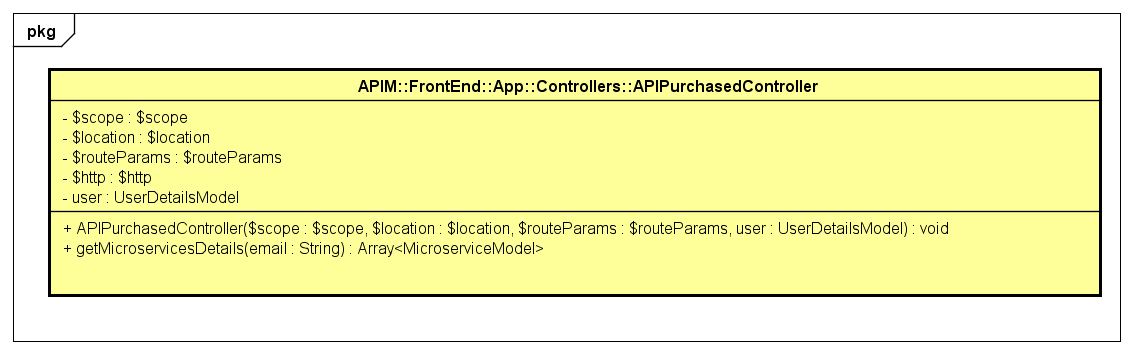
\includegraphics
	[width=0.7\linewidth]
	{images/APIM/FrontEnd/Controllers/APIPurchasedController.png}
	\caption{APIM::FrontEnd::App::Controllers::APIPurchasedController}
\end{figure}

\begin{itemize}
	\item \textbf{Descrizione:} APIPurchasedController permette di visualizzare la lista delle API comprate dall'utente ed accederne alla pagina delle informazioni dettagliate di ciascuna.
	\item \textbf{Attributi:}
		\begin{itemize}
		
			\item \textbf{\$scope : \$scope}\\
			Campo dati contenente un riferimento all'oggetto \$scope creato da AngularJS, viene utilizzato come mezzo di comunicazione tra il controller e la view. Contiene gli oggetti che definiscono il model dell'applicazione;
			
			\item \textbf{\$routeParams : \$routeParams}\\
			Parametro contenente il riferimento all'oggetto globale \$routeParams creato da AngularJS. Tale servizio permette di recuperare il set di variabili presenti nell'URL.
			
			\item \textbf{\$rootScope : \$rootScope}\\
			Campo dati contenente il riferimento all'oggetto globale \$rootScope creato da AngularJS. Viene utilizzato per rendere accessibile a tutti i controllers e a tutte le views gli oggetti MicroserviceModel e TransactionModel;
			
			\item \textbf{\$location : \$location}\\
			Campo dati contenente un riferimento al servizio creato da AngularJS che permette di accedere alla barra degli indirizzi del browser, i cambiamenti all'URL nella barra degli indirizzi si riflettono in questo oggetto e viceversa;

			\item \textbf{\$http : \$http }\\
			Campo dati che contiene un riferimento al servizio \$http che permette la comunicazione con il protocollo HTTP;
				
			\item \textbf{microservice : MicroserviceModel }\\
			Campo dati che si riferisce alla classe che rappresenta il modello di un microservizio.
			
			\item \textbf{transaction : TransactionModel }\\
			Campo dati che si riferisce alla classe che rappresenta il modello di una transazione.
				
		\end{itemize}
	\item \textbf{Metodi:}
		\begin{itemize}
		
			\item \textbf{APIPurchasedController(\$scope : \$scope, \$location : \$location, \$routeParams : \$routeParams, user : UserDetailsModel) : void}\\
			Metodo costruttore della classe.
			\begin{description}
    			\item[\textbf{Parametri:}]
			\end{description}
			\begin{itemize}
				\item \textbf{\$scope}\\
				Parametro che contiene un riferimento all'oggetto \$scope di AngularJS, impiegato nella comunicazione tra i rispettivi view e controller. Contiene gli oggetti che definiscono i model dell'applicazione;
				
				\item \textbf{\$location}\\
				Parametro che contiene un riferimento al servizio di AngularJS che permette di accedere alla barra degli indirizzi del browser, così da controllarne i cambiamenti;
			
				\item \textbf{\$routeParams}\\
				Parametro che contiene il riferimento all'oggetto globale \$routeParams di AngularJS. Permette di recuperare il set di variabili presenti nell'url;
				
				\item \textbf{user}\\
				Parametro che rappresenta un utente.
			\end{itemize}
			
			\item \textbf{getMicroservicesDetails(email : string) : Array<MicroserviceModel>}\\
			Metodo per visualizzare le informazioni dei microservizi comprati dall'utente. Si serve di un'operazione di un servizio esposto dal package \textbf{Services}.
			\begin{description}
    			\item[\textbf{Parametri:}]
			\end{description}
			\begin{itemize}
				\item \textbf{email}\\
				Parametro che rappresenta un indirizzo email.
			\end{itemize}
			
		\end{itemize}
	\item \textbf{Relazioni con altre classi:}
		\begin{itemize}
			\item Ricava i dati necessari dal package \textbf{Services};
			\item Gestisce il funzionamento della view \textbf{APIPurchased};
			\item Il model \textbf{MicroserviceModel} che contiene le informazioni per rappresentare un microservizio.
		\end{itemize}
\end{itemize}

% Fine controllers

\subsection{APIM::FrontEnd::App::node\_modules}

\subsubsection{Informazioni generali}

\begin{figure}[H]
	\centering
	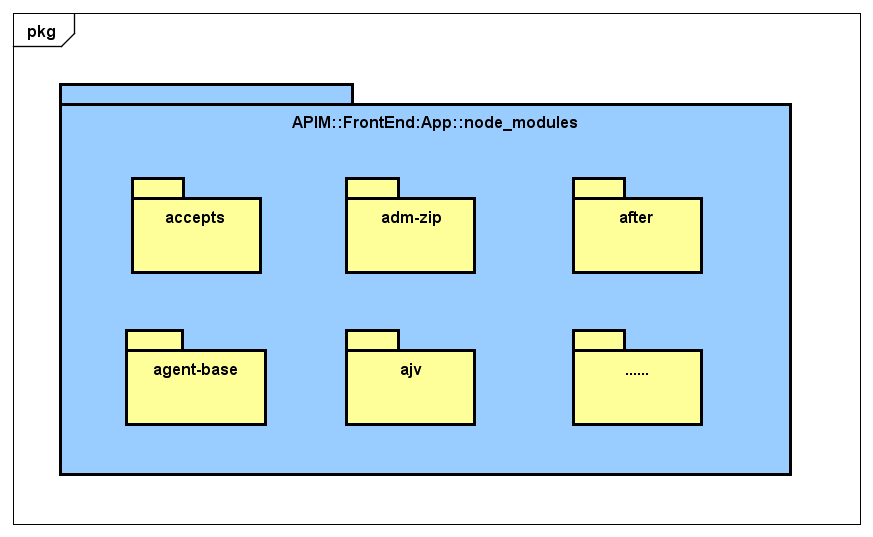
\includegraphics
	[width=0.7\linewidth]
	{images/APIM/FrontEnd/NodeModules.png}
	\caption{APIM::FrontEnd::App::node\_modules}
\end{figure}

\begin{itemize}
	\item \textbf{Descrizione:} Il package \textit{node\_modules} contiene tutti i moduli che Node.js mette a disposizione e che possono essere utilizzati dall'applicazione web.
\end{itemize}

%fine node modules